%%% The main file. It contains definitions of basic parameters and includes all other parts.

%% Settings for single-side (simplex) printing
% Margins: left 40mm, right 25mm, top and bottom 25mm
% (but beware, LaTeX adds 1in implicitly)
\documentclass[12pt,a4paper]{report}
\setlength\textwidth{145mm}
\setlength\textheight{247mm}
\setlength\oddsidemargin{15mm}
\setlength\evensidemargin{15mm}
\setlength\topmargin{0mm}
\setlength\headsep{0mm}
\setlength\headheight{0mm}
% \openright makes the following text appear on a right-hand page
\let\openright=\clearpage

%% Settings for two-sided (duplex) printing
% \documentclass[12pt,a4paper,twoside,openright]{report}
% \setlength\textwidth{145mm}
% \setlength\textheight{247mm}
% \setlength\oddsidemargin{14.2mm}
% \setlength\evensidemargin{0mm}
% \setlength\topmargin{0mm}
% \setlength\headsep{0mm}
% \setlength\headheight{0mm}
% \let\openright=\cleardoublepage

%% Generate PDF/A-2u
\usepackage[a-2u]{pdfx}

%% Character encoding: usually latin2, cp1250 or utf8:
% \usepackage[utf8]{inputenc} % turned this off after switching to xelatex in rstudio

%% Prefer Latin Modern fonts
% \usepackage{lmodern}

%% Further useful packages (included in most LaTeX distributions)
\usepackage{amsmath}        % extensions for typesetting of math
\usepackage{amsfonts}       % math fonts
\usepackage{amsthm}         % theorems, definitions, etc.
\usepackage{bbding}         % various symbols (squares, asterisks, scissors, ...)
\usepackage{bm}             % boldface symbols (\bm)
\usepackage{graphicx}       % embedding of pictures
\usepackage{fancyvrb}       % improved verbatim environment
\usepackage{natbib}         % citation style AUTHOR (YEAR), or AUTHOR [NUMBER]
\usepackage[nottoc]{tocbibind} % makes sure that bibliography and the lists
			    % of figures/tables are included in the table
			    % of contents
\usepackage{dcolumn}        % improved alignment of table columns
\usepackage{booktabs}       % improved horizontal lines in tables
\usepackage{paralist}       % improved enumerate and itemize
\usepackage{xcolor}         % typesetting in color
\usepackage{multirow}       % package for making table layouts
\usepackage{CJK}            % package for chinese, japanese, and korean symbols
\usepackage{bbold}
\usepackage{listings}
\usepackage{graphicx}
\usepackage{subcaption}
%\usepackage{nomencl}       % maybe used for abbreviations
%\makenomenclature          % maybe used for abbreviations

%%% Basic information on the thesis

% Thesis title in English (exactly as in the formal assignment)
\def\ThesisTitle{Active learning in E-Commerce Merchant Classification using Website Information}

% Author of the thesis
\def\ThesisAuthor{Mitchell Borchers}

% Year when the thesis is submitted
\def\YearSubmitted{2023}

% Name of the department or institute, where the work was officially assigned
% (according to the Organizational Structure of MFF UK in English,
% or a full name of a department outside MFF)
\def\Department{Department of Theoretical Computer Science and Mathematical Logic}

% Is it a department (katedra), or an institute (ústav)?
\def\DeptType{Department}

% Thesis supervisor: name, surname and titles
\def\Supervisor{Mgr.\ Marta Vomlelová, Ph.D.}

% Supervisor's department (again according to Organizational structure of MFF)
\def\SupervisorsDepartment{Department of Theoretical Computer Science and Mathematical Logic}

% Study programme and specialization
\def\StudyProgramme{Artificial Intelligence}
\def\StudyBranch{IUIPA}

% An optional dedication: you can thank whomever you wish (your supervisor,
% consultant, a person who lent the software, etc.)
\def\Dedication{%
I would like to thank my supervisor, Mgr.\ Marta Vomlelová, Ph.D., for her guidance throughout the duration of my thesis, as well as Adam Dobiáš and his team for the opportunity to work on this project. Additionally, I extend a big thank you to my parents, Daniel and Mary, and sisters for their unending support and encouragement.}

% Abstract (recommended length around 80-200 words; this is not a copy of your thesis assignment!)
\def\Abstract{%s
Data and the collection and analysis of data plays an important role in everyday life even though it often goes unseen. In our case, our partner is using data to classify websites into different categories. We used active learning and other machine learning methods to help classify websites into these categories and to explore the data collection and classification process. We scraped text data from websites, translated the data to English, and then worked with machine learning tools to understand the data and classify it. We found that the xPAL active learning strategy and linear support vector classifers seemed to perform best with our data.}

% 3 to 5 keywords (recommended), each enclosed in curly braces
\def\Keywords{%
{active learning} {xPAL} {machine learning} {multi-class} {classification}
}

%% The hyperref package for clickable links in PDF and also for storing
%% metadata to PDF (including the table of contents).
%% Most settings are pre-set by the pdfx package.
\hypersetup{unicode}
\hypersetup{breaklinks=true}
\newcommand{\scale}{1} % scaler used with imported figures in the thesis
% Definitions of macros (see description inside)
%%% This file contains definitions of various useful macros and environments %%%
%%% Please add more macros here instead of cluttering other files with them. %%%

%%% Minor tweaks of style

% These macros employ a little dirty trick to convince LaTeX to typeset
% chapter headings sanely, without lots of empty space above them.
% Feel free to ignore.
\makeatletter
\def\@makechapterhead#1{
  {\parindent \z@ \raggedright \normalfont
   \Huge\bfseries \thechapter. #1
   \par\nobreak
   \vskip 20\p@
}}
\def\@makeschapterhead#1{
  {\parindent \z@ \raggedright \normalfont
   \Huge\bfseries #1
   \par\nobreak
   \vskip 20\p@
}}
\makeatother

% This macro defines a chapter, which is not numbered, but is included
% in the table of contents.
\def\chapwithtoc#1{
\chapter*{#1}
\addcontentsline{toc}{chapter}{#1}
}

% Draw black "slugs" whenever a line overflows, so that we can spot it easily.
\overfullrule=1mm

%%% Macros for definitions, theorems, claims, examples, ... (requires amsthm package)

\theoremstyle{plain}
\newtheorem{thm}{Theorem}
\newtheorem{lemma}[thm]{Lemma}
\newtheorem{claim}[thm]{Claim}

\theoremstyle{plain}
\newtheorem{defn}{Definition}

\theoremstyle{remark}
\newtheorem*{cor}{Corollary}
\newtheorem*{rem}{Remark}
\newtheorem*{example}{Example}

%%% An environment for proofs

\newenvironment{myproof}{
  \par\medskip\noindent
  \textit{Proof}.
}{
\newline
\rightline{$\qedsymbol$}
}

%%% An environment for typesetting of program code and input/output
%%% of programs. (Requires the fancyvrb package -- fancy verbatim.)

\DefineVerbatimEnvironment{code}{Verbatim}{fontsize=\small, frame=single}

%%% The field of all real and natural numbers
\newcommand{\R}{\mathbb{R}}
\newcommand{\N}{\mathbb{N}}

%%% Useful operators for statistics and probability
\DeclareMathOperator{\pr}{\textsf{P}}
\DeclareMathOperator{\E}{\textsf{E}\,}
\DeclareMathOperator{\var}{\textrm{var}}
\DeclareMathOperator{\sd}{\textrm{sd}}

%%% Transposition of a vector/matrix
\newcommand{\T}[1]{#1^\top}

%%% Various math goodies
\newcommand{\goto}{\rightarrow}
\newcommand{\gotop}{\stackrel{P}{\longrightarrow}}
\newcommand{\maon}[1]{o(n^{#1})}
\newcommand{\abs}[1]{\left|{#1}\right|}
\newcommand{\dint}{\int_0^\tau\!\!\int_0^\tau}
\newcommand{\isqr}[1]{\frac{1}{\sqrt{#1}}}

%%% Various table goodies
\newcommand{\pulrad}[1]{\raisebox{1.5ex}[0pt]{#1}}
\newcommand{\mc}[1]{\multicolumn{1}{c}{#1}}


% Title page and various mandatory informational pages
\begin{document}
%%% Title page of the thesis and other mandatory pages

%%% Title page of the thesis

\pagestyle{empty}
\hypersetup{pageanchor=false}
\begin{center}

\centerline{\mbox{
\includegraphics[width=166mm]{../img/logo-en}}}

\vspace{-8mm}
\vfill

{\bf\Large MASTER THESIS}

\vfill

{\LARGE\ThesisAuthor}

\vspace{15mm}

{\LARGE\bfseries\ThesisTitle}

\vfill

\Department

\vfill

{
\centerline{\vbox{\halign{\hbox to 0.45\hsize{\hfil #}&\hskip 0.5em\parbox[t]{0.45\hsize}{\raggedright #}\cr
Supervisor of the master thesis:&\Supervisor \cr
\noalign{\vspace{2mm}}
Study programme:&\StudyProgramme \cr
\noalign{\vspace{2mm}}
Study branch:&\StudyBranch \cr
}}}}

\vfill

% Zde doplňte rok
Prague \YearSubmitted

\end{center}

\newpage

%%% Here should be a bound sheet included -- a signed copy of the "master
%%% thesis assignment". This assignment is NOT a part of the electronic
%%% version of the thesis. DO NOT SCAN.

%%% A page with a solemn declaration to the master thesis

\openright
\hypersetup{pageanchor=true}
\pagestyle{plain}
\pagenumbering{roman}
\vglue 0pt plus 1fill

\noindent
I declare that I carried out this master thesis independently, and only with the cited
sources, literature and other professional sources. It has not been used to obtain another
or the same degree.

\medskip\noindent
I understand that my work relates to the rights and obligations under the Act No.~121/2000 Sb.,
the Copyright Act, as amended, in particular the fact that the Charles
University has the right to conclude a license agreement on the use of this
work as a school work pursuant to Section 60 subsection 1 of the Copyright~Act.

\vspace{10mm}

\hbox{\hbox to 0.5\hsize{%
In \hbox to 6em{\dotfill} date \hbox to 6em{\dotfill}
\hss}\hbox to 0.5\hsize{\dotfill\quad}}
\smallskip
\hbox{\hbox to 0.5\hsize{}\hbox to 0.5\hsize{\hfil Author's signature\hfil}}

\vspace{20mm}
\newpage

%%% Dedication

\openright

\noindent
\Dedication

\newpage

%%% Mandatory information page of the thesis

\openright

\vbox to 0.5\vsize{
\setlength\parindent{0mm}
\setlength\parskip{5mm}

Title:
\ThesisTitle

Author:
\ThesisAuthor

\DeptType:
\Department

Supervisor:
\Supervisor, \SupervisorsDepartment

Abstract:
\Abstract

Keywords:
\Keywords

\vss}

\newpage

\openright
\pagestyle{plain}
\pagenumbering{arabic}
\setcounter{page}{1}


%%% A page with automatically generated table of contents of the master thesis

\tableofcontents

%%% Each chapter is kept in a separate file
\chapter*{Introduction}
\addcontentsline{toc}{chapter}{Introduction}

One of the main challenges of creating a successful machine learning model is obtaining labeled data. With easy access to a variety of modern tools, devices, and sensors, we are able to rapidly collect unlabeled data. But, in supervised learning, prediction models are trained using labeled data. The problem is that acquiring labels for the collected data can be expensive, time-consuming, or even impossible in some cases.  

However, methods have been developed to help reduce the number of labeled data required to train the classifier. Active learning is a semi-supervised machine learning framework where the model is trained with a smaller set of labeled data but which also aims to exploit trends within the unlabeled data. Active learning is a framework in which the learner has the freedom to select which data points are added to its training set (\cite{roy2001eer}). 

Active learning is different from other frameworks because it uses the unlabeled data and some evaluation criteria to determine which candidate could be the most beneficial to the model if it was given a label. In summary, the model requests the label from some oracle that provides the label then it takes this new labeled data point and rebuilds the classifier. We describe it as semi supervised active learning because of the oracle (typically a human) involved in the process that provides the label for the requested candidate data. 

In our case we will provide a set of labeled data to the active learning framework (or sampling strategy). The sampling strategy will assume all the data is unlabeled and then choose a candidate from unlabeled data pool. Then the label is revealed and the classifier is updated using the new data point.

In our case we have some data (website urls) for some company or business that are given to us from our partner. From this data our partner currently utilizes human labor to browse the website and then label the url with a category (~23 labels) and a sub-category (~234+ tags) that branch from the main category but still have some relation. This is a repetitive and expensive task that could be automated using active learning.

To reduce the burden of human labeling we propose using a combination of tools, namely, Scrapy, Postgres, translation services, and semi supervised active learning that require occasional interaction where a human can label a candidate (if unlabeled) that is expected to be most beneficial to the classifier. 

A website is required as input, then we use Scrapy to navigate to the webpage, collect and store the scraped data into the database. Next we access the data, translate the text, and add the translated data back into the database. We then create the model using the data from the database. 

In the first section we introduce active learning and the different components of active learning. In the second and third sections we discuss the details of xPAL and the process of collecting and preparing the data, respectively. In the fourth section we look at combinations of different sampling strategies / classifiers and their performance results.

\section*{Notable Definitions}

In this section we define some terms and ideas that will be helpful in understanding the upcoming sections.

\begin{defn}[Beta Prior]
\label{def:beta_prior}
A beta prior is a conjugate prior for the binomial distribution. It is a continuous probability distribution defined on the interval [0, 1] and is parameterized by two positive shape parameters, \(\alpha\) and \(\beta\). The beta distribution is defined as: 
\[\text{Beta}(\alpha, \beta) = \frac{\Gamma(\alpha + \beta)}{\Gamma(\alpha)\Gamma(\beta)}x^{\alpha - 1}(1 - x)^{\beta - 1}\]
where \(\Gamma\) is the gamma function and \(x\) is a random variable.
\end{defn}

\begin{defn}[Conjugate Prior]
\label{def:conjugate_prior}
A conjugate prior is a prior distribution that has the same functional form as the likelihood function. In other words, the posterior distribution will have the same functional form as the prior distribution.
\end{defn}

\begin{defn}[Decision-Theoretic]
\label{def:decision_theoretic}
Decision-theoretic active learning is a framework that uses the expected performance gain of a candidate to determine which candidate to label. The expected performance gain is the expected performance of the classifier after labeling the candidate minus the expected performance of the classifier before labeling the candidate. The expected performance of the classifier is the expected value of the performance measure given the posterior distribution of the classifier.
\end{defn}

\begin{defn}[Dirichlet Distribution]
\label{def:dirichlet_distribution}
The Dirichlet distribution is a multivariate generalization of the beta distribution. It is a continuous probability distribution defined on the \(K\)-simplex, \(\Delta_K = \{x \in \mathbb{R}^K: x_i \geq 0, \sum_{i=1}^K x_i = 1\}\). The Dirichlet distribution is parameterized by a vector of positive shape parameters, \(\alpha = (\alpha_1, \alpha_2, \dots, \alpha_K)\). The Dirichlet distribution is defined as:
\[\text{Dir}(\alpha) = \frac{\Gamma(\sum_{i=1}^K \alpha_i)}{\prod_{i=1}^K \Gamma(\alpha_i)}\prod_{i=1}^K x_i^{\alpha_i - 1}\]
where \(\Gamma\) is the gamma function and \(x\) is a random vector. The gamma function is defined as:
\[\Gamma(x) = \int_0^\infty t^{x - 1}e^{-t}dt\]
The gamma function is used as a normalizing constant to ensure that the probability density function integrates to 1 over the simplex, which is the space of all probability vectors that sum to 1.
\end{defn}

\begin{defn}[Ground Truth]
\label{def:ground_truth}
Ground truth is the true label of a data point.
\end{defn}

\begin{defn}[Posterior Probabilities]
\label{def:posterior_probabilities}
Posterior probability is a type of conditional probability that results from updating the prior probability with information summarized by the likelihood via an application of Bayes' rule. The posterior probability is the probability of an event occurring given that another event has occurred.
\end{defn}

\begin{defn}[Omniscient Oracles]
\label{def:omniscient_oracles}
Omniscient oracle is a hypothetical entity that has complete knowledge of the true labels of all data points in a given dataset. An omniscient oracle knows the ground truth labels of all data points.
\end{defn}


\chapter*{Definitions}
\addcontentsline{toc}{chapter}{Definitions}

In this section we define some terms and ideas that will be helpful in understanding the upcoming sections.

\begin{defn}[Beta Prior]
\label{def:beta_prior}
A beta prior is a conjugate prior for the binomial distribution. It is a continuous probability distribution defined on the interval [0, 1] and is parameterized by two positive shape parameters, \(\alpha\) and \(\beta\). The beta distribution is defined as: 
\[\text{Beta}(\alpha, \beta) = \frac{\Gamma(\alpha + \beta)}{\Gamma(\alpha)\Gamma(\beta)}x^{\alpha - 1}(1 - x)^{\beta - 1}\]
where \(\Gamma\) is the gamma function and \(x\) is a random variable. The gamma function is defined as:
\[\Gamma(x) = \int_0^\infty t^{x - 1}e^{-t}dt\]
The gamma function is used as a normalizing constant to ensure that the probability density function integrates to 1 over the simplex, which is the space of all probability vectors that sum to 1.
\end{defn}

\begin{defn}[Conjugate Prior]
\label{def:conjugate_prior}
A conjugate prior is a prior distribution that is in the same family of distributions as the likelihood function. In other words, the posterior distribution will have a similar functional form to the prior distribution.
\end{defn}

\begin{defn}[Decision-Theoretic]
\label{def:decision_theoretic}
Decision-theoretic active learning is a framework that uses the expected performance gain of a candidate to determine which candidate to label. The expected performance gain is the expected performance of the classifier after labeling the candidate minus the expected performance of the classifier before labeling the candidate. The expected performance of the classifier is the expected value of the performance measure given the posterior distribution of the classifier.
\end{defn}

\begin{defn}[Dirichlet Distribution]
\label{def:dirichlet_distribution}
The Dirichlet distribution is a multivariate generalization of the beta distribution. It is a continuous probability distribution defined on the \(K\)-simplex, \(\Delta_K = \{x \in \mathbbm{R}^K : x_i \geq 0, \sum_{i=1}^K x_i = 1\}\). The Dirichlet distribution is parameterized by a vector of positive shape parameters, \(\alpha = (\alpha_1, \alpha_2, \dots, \alpha_K)\). The Dirichlet distribution is defined as:
\[\text{Dir}(\alpha) = \frac{\Gamma(\sum_{i=1}^K \alpha_i)}{\prod_{i=1}^K \Gamma(\alpha_i)}\prod_{i=1}^K x_i^{\alpha_i - 1}\]
where \(\Gamma\) is the gamma function as defined in Definition \ref{def:beta_prior} and where \(x\) is a random vector.
\end{defn}

\begin{defn}[Ground Truth]
\label{def:ground_truth}
Ground truth is the true label of a data point.
\end{defn}

\begin{defn}[Posterior Probabilities]
\label{def:posterior_probabilities}
Posterior probability is a type of conditional probability that results from updating the prior probability with information summarized by the likelihood via an application of Bayes' rule. The posterior probability is the probability of an event occurring given that another event has occurred.
\end{defn}

\begin{defn}[Omniscient Oracles]
\label{def:omniscient_oracles}
Omniscient oracle is a hypothetical entity that has complete knowledge of the true labels of all data points in a given dataset. An omniscient oracle knows the ground truth labels of all data points.
\end{defn}

\begin{defn}[TF-IDF]
\label{def:tf_idf}
TF-IDF is a numerical statistic that is intended to reflect how important a word is to a document in a collection or corpus. It is often used as a weighting factor in information retrieval and text mining. The TF-IDF value increases proportionally to the number of times a word appears in the document and is offset by the frequency of the word in the corpus (large structured set or collection of speech or text data).
\end{defn}
\chapter{Active Learning}



\section{Introduction}
Russel and Norvig succinctly define an agent and different types of learning in their book "Artificial Intelligence: A Modern Approach" (\cite{russell2009artificial}), their definition is paraphrased here. They define an agent as something that acts and a rational agent as one that acts so as to achieve the best outcome. If there there is uncertainty, then the agent tries to achieve the best expected outcome. Any component of an agent can be improved by learning from data. The improvements and techniques used to make them depend on four major factors:

\begin{itemize}
  \item Which component is to be improved.
  \item What prior knowledge the agent already has.
  \item What representation is used for the data and the component.
  \item What feedback is available to learn from.  
\end{itemize}

Here we will mostly be focused on the final point, "What feedback is available to learn from". However, we will also discuss the importance of the second and third points because of our use of Bayesian learning and how the form and quality of the data affects the experiments. There are three main types of feedback that determine the three main types of learning which are unsupervised, reinforcement, and supervised learning. 

In unsupervised learning an agent learns patterns even though no feedback is provided. In reinforcement learning, the agent learns from a series of rewards or punishments. In supervised learning, an agent learns from input-output pairs, which can be discrete or continuous, to find a function that maps the pairs. 

The goal of supervised learning is given a training set of $N$ example input-output pairs:

\[(x_1, y_1), (x_2,y_2),... (x_N,y_N),\]

where each $y_j$ was generated by some unknown function $y=f(x)$, find a function $h$ that approximates the true function.

In reality, the lines separating the types of learning aren't so clear. Semi-supervised learning is also an important and widely used method. In semi-supervised learning we are given a few labeled examples that were labeled by some oracle (labeler, data annotator, etc.) and we must then make the most of a large collection of unlabeled examples. But what can we do with the unlabeled data? 

Supervised learning models almost always get more accurate with more labeled data. Active learning is the process of deciding which data to select for annotation (\cite{munro2021human}). In other words, the central component of an active learning algorithm is the selection strategy, or deciding which of the unlabeled data could be the most useful to the model if it was labeled. Active learning uses a selection strategy that augments the existing classifier, it is not itself a classifier but rather a tool paired with a classifier.

Many strategies for choosing the next points to label exist. First we will discuss query functions then we will briefly define three basic sampling approaches: uncertainty, diversity, and random sampling to get an idea of sampling. We will then discuss some more advanced sampling approaches that are used in our experiments. When sampling the unlabeled data an ordered list is returned and the top candidate is the candidate that is expected to be most valuable for the model, but we are not strictly limited to taking just one candidate.

\section{Query Function Construction}
There are various techniques used to construct the querying functions we have discussed. We will focus on pool-based active learning, but a number of interesting and relevant ideas appear within other active-learning frameworks that are worth mentioning.

\subsection{Pool-Based}
The learner calculates the potential gain of all the unlabeled points in the pool, then requests the label for the point that maximizes the expected information gain for the classifier (\cite{huang2016alce}). For pool-based multiclass active learning, a labeled pool and an unlabeled pool are presented to the algorithm. In each iteration, the algorithm selects one instance from the unlabeled pool to query its label.

\subsection{Stream-Based}
The learner is provided with a stream of unlabeled points. On each trial, a new unlabeled point is drawn and introduced to the learner who must decide whether or not to request its label (\cite{baram2004online}). Note that the stream-based model can be viewed as an online version of the pool-based model. 

\subsection{Membership Queries}
On each trial the learner constructs a point in input space and requests its label (\cite{baram2004online}). This model can be viewed as a pool-based game where the pool consists of all possible points in the domain.

\section{Sampling Strategies}

Sampling strategies, also referred to as selection strategies, are the core of the active learning process. The goal of sampling is to select the most useful data points from the unlabeled pool to label. The most useful data points are those that are expected to improve the classifier the most.

\subsection{Random Sampling}
Random sampling is self explanatory as it randomly selects an unlabeled data point from the pool and requests to have it labeled then used in the model.

\subsection{Diversity Sampling}
Diversity sampling is the set of strategies for identifying unlabeled items that are underrepresented or unknown to the machine learning model in its current state (\cite{munro2021human}). The items may have features that are unique or obscure in the training data, or they might represent data that are currently under-represented in the model. 

Either way this can result in poor or uneven performance when the model is applied or the data is changing over time. The goal of diversity sampling is to target new, unusual, or underrepresented items for annotation to give the algorithm a more complete picture of the problem space. 

\subsection{Uncertainty Sampling}
Uncertainty sampling is the set of strategies for identifying unlabeled items that are near a decision boundary in the current machine learning model (\cite{munro2021human}). Uncertainty sampling is simple given a classifier that estimates $P (C|w)$ (\cite{lewis1994uncertainty}). On each iteration, the current version of classifier can be applied to each data point, and the data with estimated $P(C|w)$ values closest to 0.5 are selected, since 0.5 corresponds to the classifier being most uncertain of the class label.

These items are most likely to be wrongly classified, so they are the most likely to result in a label that differs from the predicted label, moving the decision boundary after they have been added to the training data and the model has been retrained.

\subsection{PAL}
Probabilistic Active Learning (PAL) follows a smoothness assumption and models for a candidate instance both the true posterior in its neighborhood and its label as random variables (\cite{kottke2014pal}). By computing for each candidate its expected gain in classification performance over both variables, PAL selects the candidate for labeling that is optimal in expectation. PAL shows comparable or better classification performance than error reduction and uncertainty sampling, has the same asymptotic linear time complexity as uncertainty sampling, and is faster than error reduction.

\subsection{xPAL}
Extended probabilistic gain for active learning (xPAL) is a decision-theoretic selection strategy that directly optimizes the gain and misclassification error, and uses a Bayesian approach by introducing a conjugate prior distribution to determine the class posterior to deal with uncertainties (\cite{kottke2021toward}). Although the data distribution can be estimated, there is still uncertainty about the true class posterior probabilities. 

These class posterior probabilities can be modeled as a random variable based on the current observations in the dataset. For this model, a Bayesian approach is used by incorporating a conjugate prior to the observations. This produces more robust usefulness estimates for the candidates.

\subsection{ALCE}
Active Learning with Cost Embedding (ALCE) is a non-probabilistic uncertainty sampling algorithm for cost-sensitive multiclass active learning (\cite{huang2016alce}). They first designed a cost-sensitive multiclass classification algorithm called cost embedding (CE), which embeds the cost information in the distance measure in a special hidden space by non-metric multidimensional scaling. They then use a mirroring trick to let CE embed the possibly asymmetric cost information in the symmetric distance measure.

\subsection{QBC}
Query by committee uses an ensemble of classifiers that are trained on bootstrapped replicates of the labeled set (\cite{seung1992qbc}). The idea is to train a committee of classifiers on the available labeled data and then use the committee to select the most informative unlabeled data for labeling (\cite{freund1997qbc}). The committee consists of several classifiers, each trained on a slightly different subset of the available labeled data.

The QBC algorithm measures the disagreement of the committee's predictions on each unlabeled data point. The intuition is that if the committee members disagree then it is likely to be a difficult data point for the current classifier and thus informative for labeling.

The algorithm selects a fixed number of the most informative examples and asks the user or oracle to label them. The labeled examples are then added to the labeled dataset, and the committee is retrained on the expanded labeled dataset. This process is repeated until the algorithm achieves a desired level of accuracy or the available labeling budget is exhausted.

\subsection{EER}
Monte Carlo estimation of error reduction (EER) estimates future error rate by log-loss, using the entropy of the posterior class distribution on a sample of the unlabeled examples, or by 0-1 loss, using the posterior probabilities of the most probable class for the sampled unlabeled examples (\cite{roy2001eer}).

\section{Classifiers}

The main classifier used with the active learning sampling strategies is the Parzen Window Classifier (PWC). It is a non-parametric method used for classification and density estimation in machine learning. It works by estimating the probability density function of a given class using a kernel density estimator, and then using Bayes' theorem to classify new instances based on their estimated probability densities.

We will also explore using other classifiers from Scikit-Learn and TensorFlow and compare their performance on the data without using active learning to see if there is any improvement beyond the PWC classifier.

\section{Summary}
Now it should be more clear how the sampling strategy is the major component of active learning. The query function construction is also important but it is just a means of routing the data to be sampled. In the next chapter we will look into the specifics of xPAL.

\chapter{Understanding xPAL}

We have introduced many different active learning models in the previous section, and we will test some of these models on our data. However, we will mainly focus on using the xPAL sampling strategy and a pool based query function. The xPAL sampling strategy is a decision-theoretic approach to measure the usefulness of a labeling candidate in terms of its expected performance gain (\cite{kottke2021toward}). We can estimate the data distribution but we are uncertain about the true class posterior probabilities. The class posterior probabilities are modeled as a random variable based on the current observations. Therefore a Bayesian approach is used by incorporating a conjugate prior to the observations. In general, the idea is to estimate the expected performance gain for the classifier, using the unlabeled data, and then select the best data point and request its label. Variable descriptions used in the following equations and explanations are listed in Table \ref{tab:var_defs}

\begin{table}[ht]
\centering
\begin{tabular}{|l|l|}
\hline
{} & \textbf{Descriptions} \\
\hline
$C$                         & Number of classes \\
\hline
$x$                         & Input $x \in \mathbb{R}^n$\\
\hline
$y$                         & Output $y \in l_1,...,l_C$ \\
\hline
$\textit{L}$                & Loss ??\\
\hline
$\textit{R}$                & Risk $\textit{R}(f^{\mathcal{L}}) \in \mathbb{R}_0^x$ \\
\hline
$\textit{R}_{\mathcal{E}}$  & Empirical risk ??\\
\hline
$\mathcal{L}$               & Set of labeled data $\{(x_1,y_1),...,(x_n,y_n)\}$ \\
\hline
$\mathcal{U}$               & Set of unlabeled data $\{x_1,...,x_n\}$ \\
\hline
$\mathcal{E}$               & Set of labeled and unlabeled data \\
\hline
$p(x,y)$                    & Joint distribution of random variables $x$ and $y$ \\
\hline
$f^{\mathcal{L}}$           & Classifier that maps input $x$ to output $y$ \\
\hline
\end{tabular}
\caption{Variable names and definitions.}
\label{tab:var_defs}
\end{table}

\section{Kernel}

A kernel based classifier is used in xPAL which determines the similarity of two data points. The kernel function $\textbf{\textit{K}}(x,x')$ is a function that maps two data points to a real number. The kernel frequency estimate $\textbf{\textit{k}}^{\mathcal{L}}_x$ of an instance $\textbf{\textit{x}}$ is calculated using the labeled instances $\mathcal{L}$. The y-th element of that C-dimensional vector describes the similarity-weighted number of labels of class y.

\begin{equation}
\textbf{\textit{k}}^{\mathcal{L}}_x,y = \sum_{(x',y') \in \mathcal{L}} \mathbb{1}_{y=y'} \textbf{\textit{K}}(x,x')
\label{eq:kernel}
\end{equation}

The Parzen Window Classifier uses the labeled data for training and predicts the most frequent class. 

\begin{equation}
f^{\mathcal{L}}(x) = \underset{y \in \mathcal{Y}}{\arg \max} \left( \textbf{\textit{k}}^{\mathcal{L}}_{x,y} \right) \hbox{.}
\end{equation}

We will mainly use the PWC classifier in our experiments but we will also evaluate other classifiers and compare their performance.

\section{Risk}

For xPAL, Kottke et al. use the classifications error as the performance measure and minimize the zero-one loss. The risk describes the expected value of the loss relative to the joint distribution given some classifier. The zero-one loss returns 0 if the prediction from the classifier is equal to the true class else it returns 1. The risk is a theoretical concept that cannot be computed directly since it requires knowledge of the entire population distribution. Instead, we typically try to approximate the risk using the empirical risk.

\begin{flalign}
\textit{R}(f^{\mathcal{L}}) &= \underset{p(x,y)}{\mathbb{E}} [ \textbf{\textit{L}}(y,f^{\mathcal{L}}(x)) ] \\
&= \underset{p(x)}{\mathbb{E}} \left[ \underset{p(y|x)}{\mathbb{E}} [ \textbf{\textit{L}}(y,f^{\mathcal{L}}(x)) ] \right] \\
\textbf{\textit{L}}(y,f^{\mathcal{L}}(x)) &= \mathbb{1}_{f^{\mathcal{L}}(x)\neq y} 
\end{flalign}

Because it is not known how the data is generated Kottke et al. use a Monte-Carlo integration with all the data $\mathcal{E}$ to represent the generator. The empirical risk $\textit{R}_{\mathcal{E}}$ is the average of the loss over all the data points in the dataset. It refers to the average value of a given loss function over a finite set of observed data points. The empirical risk is a computable quantity that can be used as an estimate of the risk. However, it is only an approximation and is subject to sampling error.

\begin{flalign}
    \textit{R}_{\mathcal{E}}(f^{\mathcal{L}}) &= \frac{1}{|\mathcal{E}|} \sum_{x \in \mathcal{E}} \underset{p(y|x)}{\mathbb{E}} \left[ \textbf{\textit{L}}(y,f^{\mathcal{L}}(x)) \right] \\
    &= \frac{1}{|\mathcal{E}|} \sum_{x \in \mathcal{E}} \sum_{y \in \mathcal{Y}} p(y|x) \textbf{\textit{L}}(y,f^{\mathcal{L}}(x))
\label{eq:empirical_risk}
\end{flalign}


\section{Conjugate Prior}

The conditional class probability $p(y|x)$ depends on the ground truth which is unkown. As a result the conditional class probability is exactly the y-th element of the unknown ground truth vector $\textit{\textbf{p}}$. The nearby labels from $\mathcal{L}$ can be used to estimate the ground truth $\textit{\textbf{p}}$ becuase the oracle provides the labels according to $\textit{p}$. If we assume a smooth distribution then the estimate is relatively close to the ground truth if we have enough labeled instances. 

\begin{equation}
p(y|x) = p(y|t(x)) = p(y|\textit{\textbf{p}}) = \text{Cat} (y|\textbf{p}) = p_y
\end{equation}

A Bayesian approach is used for estimation by calculating the posterior predictive distribution (calculating the expected value over all possible ground truth values). The probability of y given some x is approximately equal to the kernel frequency estimate of x. 

\begin{equation}
p(y|x) \approx  p(y | \textbf{\textit{k}}^{\mathcal{L}}_x) = \underset{p(p|\textbf{\textit{k}}^{\mathcal{L}}_x)}{\mathbb{E}} \left[ p_y \right] = \int p(p|\textbf{\textit{k}}^{\mathcal{L}}_x) p_y dp
\label{eq:kernel_estimate}
\end{equation}

Bayes theorem is then used to determine the posterior probability of the ground truth at instance x in Equation \ref{eq:bayes}. The likelihood $p(\textbf{\textit{k}}^{\mathcal{L}}_x|p)$ is a multinomial distribution because each label has been drawn from $Cat(y|p)$. A prior is introduced and selected as a Dirichlet distribution with $\alpha \in \mathbb{R}^C$ as this is the conjugate prior of the multinomial distribution. An indifferent prior is choosen and each element of alpha is set to the same value. The Dirichlet distribution is an analytical solution for the posterior when the conjugate prior of the multinomial likelihood are used. 

\begin{flalign}
\label{eq:bayes}
p(p|\textbf{\textit{k}}^{\mathcal{L}}_x) &= \frac{p(\textbf{\textit{k}}^{\mathcal{L}}_x|p)p(p)}{p(\textbf{\textit{k}}^{\mathcal{L}}_x)} \\
&= \frac{\text{Mult}(\textbf{\textit{k}}^{\mathcal{L}}_x|p) \cdot \text{Dir}(p|\alpha)}{\int \text{Mult}(\textbf{\textit{k}}^{\mathcal{L}}_x|p) \cdot \text{Dir}(p|\alpha) dp} \\
&= \text{Dir}(p|\textbf{\textit{k}}^{\mathcal{L}}_x + \alpha)
\end{flalign}

The conditional class probability is determined next from Equation \ref{eq:kernel_estimate}. It is calculated with the expected value of the Dirichlet distribution.

\begin{flalign}
p(y|\textbf{\textit{k}}^{\mathcal{L}}_x) &= \underset{\text{Dir}(p|\textbf{\textit{k}}^{\mathcal{L}}_x+ \alpha)}{\mathbb{E}} \left[ p_y \right] \\
&= \int \text{Dir}(p|\textbf{\textit{k}}^{\mathcal{L}}_x + \alpha) p_y dp \\
&= \frac{\textbf{(\textit{k}}^{\mathcal{L}}_x + \alpha)_y}{||\textbf{\textit{k}}^{\mathcal{L}}_x + \alpha ||_1}
\label{eq:cond_class_prob}
\end{flalign}

The last term is the y-th element of the normalized vector. The 1-norm is used to normalize the vector.

\section{Risk Difference Using the Conjugate Prior}

Next, we insert equation \ref{eq:cond_class_prob} into the empirical risk equation \ref{eq:empirical_risk}. We are approximating $p(y|x)$ with $p(y|\textbf{\textit{k}}_x^\mathcal{L})$ which is the empirical risk based on the labeled data $\mathcal{L}$.

\begin{equation}
    \hat{R}_{\mathcal{E}} (f^{\mathcal{L}}, \mathcal{L}) = \frac{1}{|\mathcal{E}|} \sum_{x \in \mathcal{E}} \sum_{y \in \mathcal{Y}}  \frac{\textbf{(\textit{k}}^{\mathcal{L}}_x + \alpha)_y}{||\textbf{\textit{k}}^{\mathcal{L}}_x + \alpha ||_1} \cdot \textit{L} (y,f^{\mathcal{L}}(x))
\end{equation}

Now lets assume we add a new labeled candidate $(x_c,y_c)$ to the labeled data set $\mathcal{L}$. We will now denote the set with the newly labeled data point $\mathcal{L}^+ = \mathcal{L} \cup \{(x_c,y_c)\}$. Next we need to determine how much the how well this new data point improved our classifier. We then make an estimate of the gain in terms of risk difference using the probability to estimate the ground truth.

\begin{flalign}
    \Delta \hat{R}_{\mathcal{E}} (f^{\mathcal{L}^+}, f^{\mathcal{L}}, \mathcal{L}^+) &= \hat{R}_{\mathcal{E}} (f^{\mathcal{L}^+}, \mathcal{L}^+) - \hat{R}_{\mathcal{E}} (f^{\mathcal{L}}, \mathcal{L}^+) \\
    &= \frac{1}{|\mathcal{E}|} \sum_{x \in \mathcal{E}} \sum_{y \in \mathcal{Y}}  \frac{\textbf{(\textit{k}}^{\mathcal{L}^+}_x + \alpha)_y}{||\textbf{\textit{k}}^{\mathcal{L}^+}_x + \alpha ||_1} \cdot \left( \textit{L} (y,f^{\mathcal{L}^+}(x)) - \textit{L}(y,f^{\mathcal{L}}(x)) \right)
\label{eq:delta_emp_risk}
\end{flalign}

The observations used to estimate the risk are the same for both the old and new classifiers. We do this because we assume that adding labeled data will make the classifier better, so this allows us to more accurately compare the current classifier and the new one.

\section{Expected Probabilistic Gain}

If we are able to reduce the error with the new $\mathcal{L}^+$ model then equation \ref{eq:delta_emp_risk} will be negative. As a result, we negate this term and maximize the expected probabilistic gain. To simplify we set $\alpha = \beta$.

\begin{flalign}
    \text{xgain}(x_c, \mathcal{L}, \mathcal{E}) =& \underset{p(y_c|\textbf{\textit{k}}^{\mathcal{L}}_{x_c})}{\mathbb{E}} \left[ - \Delta \hat{R}_{\mathcal{E}} (f^{\mathcal{L}^+}, f^{\mathcal{L}}, \mathcal{L}^+ \right] \\
    =& - \sum_{y \in \mathcal{Y}}  \frac{\textbf{(\textit{k}}^{\mathcal{L}}_x + \beta)_y}{||\textbf{\textit{k}}^{\mathcal{L}}_x + \beta ||_1} \cdot \frac{1}{|\mathcal{E}|} \sum_{x \in \mathcal{E}} \sum_{y \in \mathcal{Y}} \notag \\
    & \frac{\textbf{(\textit{k}}^{\mathcal{L}^+}_x + \alpha)_y}{||\textbf{\textit{k}}^{\mathcal{L}^+}_x + \alpha ||_1} \cdot \left( \textbf{\textit{L}} (y,f^{\mathcal{L}^+}(x)) - \textbf{\textit{L}}(y,f^{\mathcal{L}}(x)) \right)
\end{flalign}

\section{xPAL Selection Strategy}

The xPAL selection strategy chooses this candidate $x^*_C \in \mathcal{U}$ where the gain is maximized:

\begin{equation}
    x^*_c = \underset{x_c \in \mathcal{U}}{\arg \max} \left( \text{xgain} (x_c, \mathcal{L}, \mathcal{E}) \right)
\end{equation}

\chapter{Related Works}

The main paper that influenced our work is called 'E-Commerce Merchant Classification using Website Information' published by \cite{sahid2019ecommerce}. In this paper the authors test different text processing strategies, embeddings, machine learning methods, and scraping methodologies. 

\section{E-commerce Merchant Classification}

The authors explaining the importance of e-commerce and the need for accurate classification of e-commerce merchants for market analysis and risk management in relation to using a payment gateway service. In their case it is important to classify a merchant to see if they are in a high risk category. They then describe the proposed method, which consists of three main stages: data collection, data preprocessing, and merchant classification.

In the collection stage, the authors collect data from e-commerce websites using a web crawler. They extract the html text data from the home page and various sibling pages, depending on the experiment.

In the preprocessing stage, the authors perform several steps to clean and transform the data. They remove missing and redundant features, characters of length 1 or 2 and sequences of numbers. Next, they use TF, TF-IDF, or embedding to create their dataset.

In the merchant classification stage, the authors apply several machine learning algorithms, including Decision Trees, Naive Bayes, k-NN, MLP, Logistic Regression, and Support Vector Machine (SVM) to classify the e-commerce merchants into several categories, such as electronics, flowers, and gambling. They evaluate the performance of each algorithm using several metrics, such as accuracy, precision, recall, and F1 score.

The experimental results show that the proposed method outperforms the baseline method in terms of classification accuracy and other metrics. The SVM algorithm achieves the highest macro averaged F-score of 0.83 indicating that the proposed method is effective in classifying e-commerce merchants based on their website data.

\section{Influence}

The e-commerce paper helped guide us in our work because we used lessons they learned to tailor our approach. For example, we focused on scraping data from just the home page and using TF-IDF instead of exploring other methods. However, we also incorporate active learning which was not used in the e-commerce paper.
\chapter{Data Review}

In this chapter we take a deeper look into the data and the process of collecting, translating, and encoding the data. Our partner has provided a small sample of 1000 labeled data points. This data was manually labeled by an human annotator. 

\section{Overview}

The data consists of a merchant name, merchant website (url), merchant category, and merchant tag as shown in Table \ref{tab:data_point}. 

\begin{table}[h]
\begin{tabular}{|l|l|l|l|}
\hline
merchant name            & merchant url            & merchant category & merchant tags           \\ \hline
State Hospital & http://hospital.com/ & Health   & '\{"Clinic"\}' \\ \hline
\end{tabular}
\caption{This is an example of a single data point from the original data set.}
\label{tab:data_point}
\end{table}


The current process consists of giving the merchant url to an annotator. The annotator then views the website and either can instantly (after viewing the homepage) provide a label and tags for the website. However, in some cases the annotator may need to browse further (by viewing sibling pages such as the 'About Us' section or individual product pages) to get an idea of how the website should be classified. 

The annotator simply needs to view then mentally process the text and images from the website and make some reasonable decisions on how the site should be classified. However, the annotator does not record what the content on the site said or what drove them to make their decision.As a result we are missing a key portion of data for the classification process. 

Tags are also when labeling the data to provide further granularity. The merchant tags are ordered by specificity, with the first tag in the list being the most general and the final being the most specific. An example of the tag hierarchy is show in Table. \ref{tab:tags} where we can see that this sample consists of data from various categories all contained within the 'Eco' side tag grouping.


\begin{table}[h]
\begin{tabular}{|l|l|l|l|l|}
\hline
Category    & Level 1 Tag           & Level 2 Tag        & Level 3 Tag  & Side Tag \\ \hline
Travel      & Local Transport       & Micro-mobility     & Bike Sharing & Eco      \\ \hline
            &                       & Public Transport   &              & Eco      \\ \hline
Fashion     & Clothing - Other      & Second Hand        &              & Eco      \\ \hline
Car         & Charging Station      &                    &              & Eco      \\ \hline
            & Car Sharing           &                    &              & Eco      \\ \hline
\end{tabular}
\caption{This is an example of how the tags use different levels.}
\label{tab:tags}
\end{table}

The tags are important because they allow us to separate the data even further and group or sort the data differently. However, in our work we didn't opt to include the tags in the classification or selection strategy process at this time.

\section{Collection}

Similarly to the annotator our goal is to automate the navigation, collection/ storing process, and classification of the website. This process speeds up the browsing process by navigating to websites that have already been labeled and scraping the text data and storing it into a database.

The initial 1000 data points we received were labels with a pointer (a url) to where the text data is located (the website). The labels needed the text from the websites that the annotator viewed to begin the classifying process. To gather the text data from the websites we used the Scrapy framework to extract text data from a single top level page of a website. We chose only to scrape the top level (main or home) page text because of the results published in another study where it was observed that adding more pages to the data set does not necessarily mean obtaining better results (\cite{sahid2019ecommerce}). 

Out of these initial data points 179 contained links that could not be accessed or links that provided no text data that could be scraped. Two websites were particularly problematic. Facebook and Instagram both are used by business as main information webpages. However, neither site allows for simple text scraping and a more advanced approach was needed to extract data from business with information on these platforms. Out of the remaining 821 data points 274 of them were in English. Out of the remaining 274 English data points the data was distributed into the categories as shown in Figure \ref{fig:original_english_counts}.

\section{Processing}

It is important for us to have the data in English as it allows us to exploit stop words when using the Scikit-Learn TF-IDF vectorizer to construct our data set. Stop words are words like “and”, “the”, “him”, which are presumed to be uninformative in representing the content of a text, and which may be removed to avoid them being construed as signal for prediction (\cite{sklearn62feature}). This holds true for our data set as well.

At this stage, it was clear that our data set wasn't representing all categories equally. The 'Food and Drink' category has many more data points then the 'Culture' and 'Investments' categories which each had a single data point, see Figure \ref{fig:original_english_counts}. The 'Children' and 'Financial Services' categories weren't represented at all. Obviously this was problematic because we would like to have, minimum, three data points in each category to build train and test sets.

\begin{figure}[!ht]
  \centering
  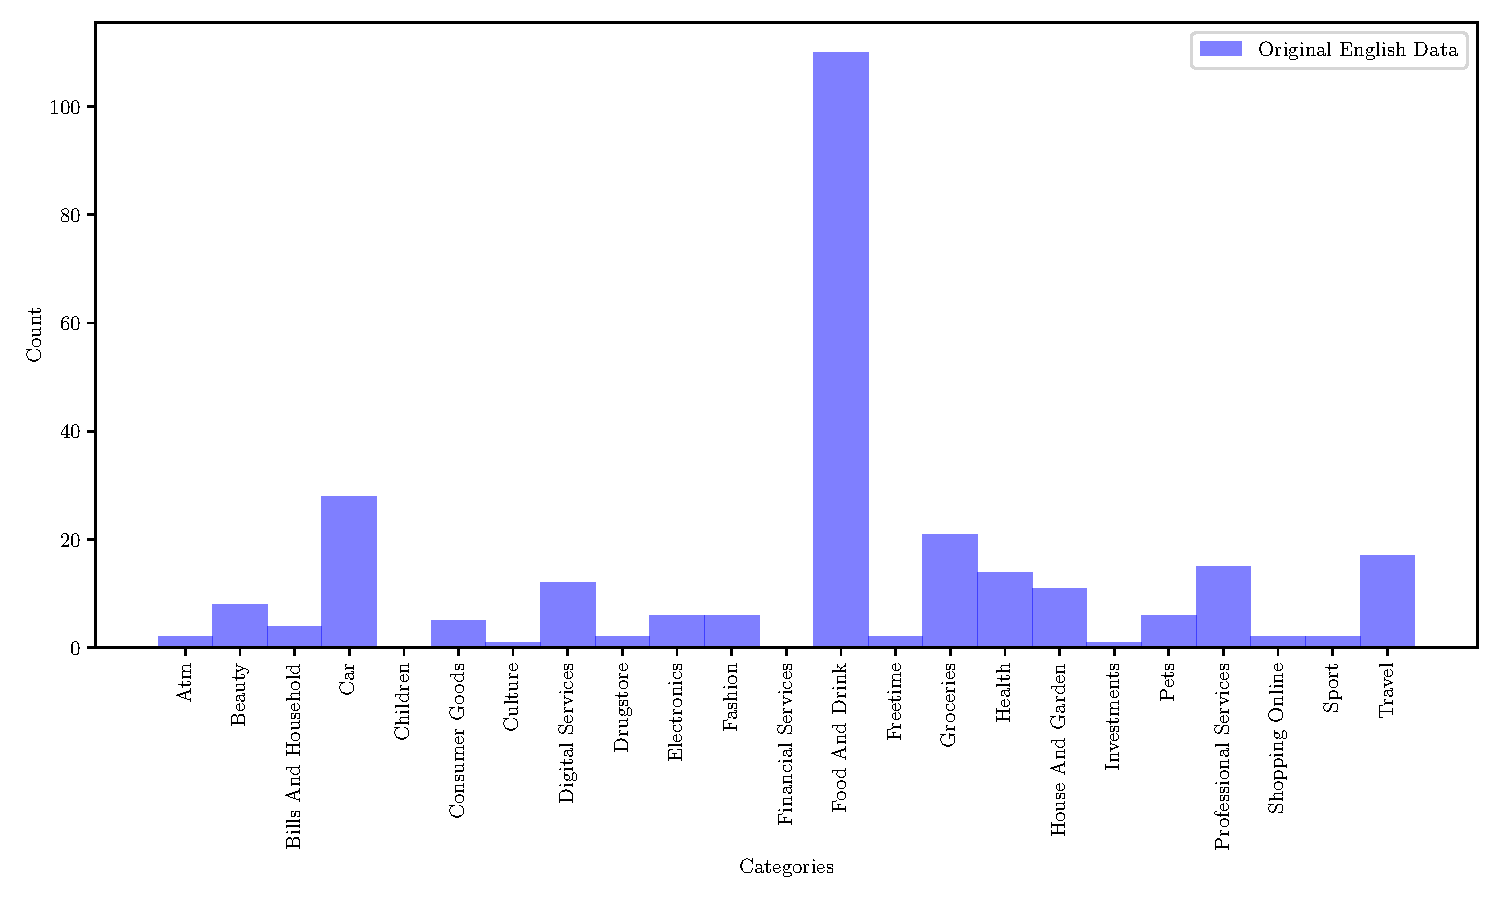
\includegraphics[width=\textwidth]{../img/plot_original_english_counts.pdf}
  \caption{The histograms for the original usable english data.}
  \label{fig:original_english_counts}
\end{figure}

At this point we had a significant amount of data that wasn't being used (the untranslated data). We decided to find a way to translate the existing data. We tried various libraries available on GitHub but weren't getting good results. We found that Azure had a service available and a free option of up to 2 million characters translated per month. This was a viable option and we were able to use this API to translate the remaining data. We limited the number of characters to 1000 per data point from the scraped text to avoid maxing out the API.

An example of the first 100 characters of raw scraped text data from a website is shown in Table \ref{tab:text_examples}. The scraped text data is a single string of text that is a concatenation of all the text data pulled from the website url. 

\begin{table}[!ht]
\centering
\caption{Raw text collected by scraper and the translated text.}
\begin{tabular}{|l|p{10cm}|}
\hline
Raw & DentalVision - Profesionální soukromá zubní klinika v centru Hradce Králové ÚvodSlužby a ceníkOrdina \\ \hline
Translated & DentalVision Professional private dental clinic in the center of Hradec Králové IntroductionServices \\ \hline
\end{tabular}
\label{tab:text_examples}
\end{table}

We can see that the symbols were removed and the majority of the words were translated. There are still some issues with words being concatenated, but we attempt to break these words apart before passing the text to the TF-IDF vectorizer.

In addition to the original data we also manually collected and labeled 141 additional data points. All the original data and additional data counts are shown in Figure \ref{fig:all_hist} and discretely in Appendix Table \ref{tab:data_counts}.


\begin{figure}[!ht]
  \centering
  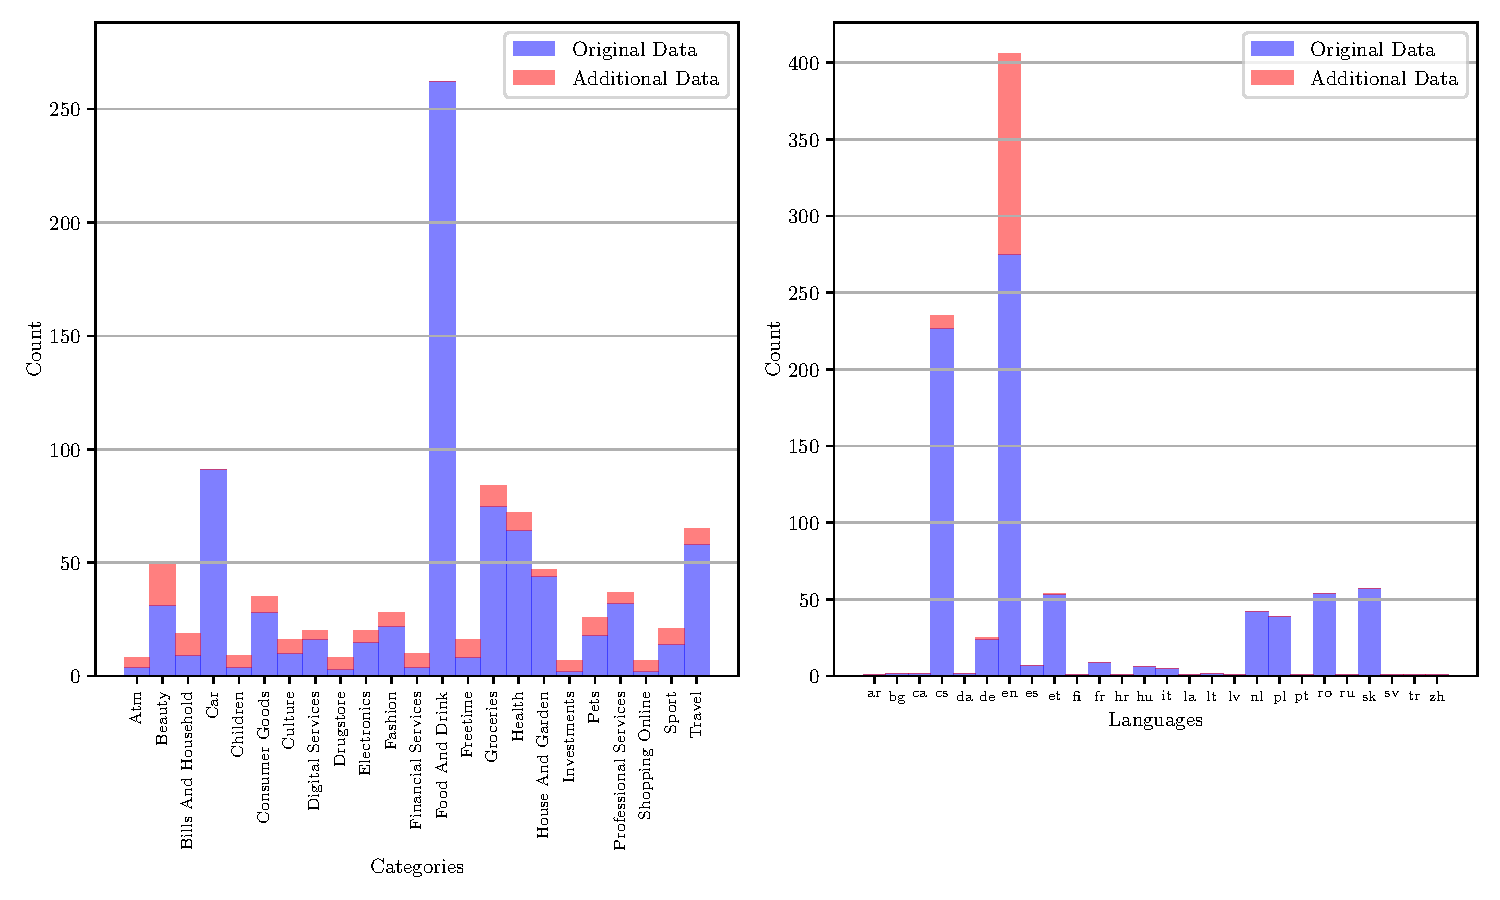
\includegraphics[width=\textwidth]{../img/plot_all_hist.pdf}
  \caption{The histograms for the original and additional data for all languages.}
  \label{fig:all_hist}
\end{figure}


After translating the data we used the TF-IDF vectorizer from Scikit-Learn. We were able to find highly correlated words for each category using Chi Squared analysis with only the original data, shown below in Table \ref{tab:correlated_unigrams_original}. Some categories such as 'Culture', 'Digital Services', 'Shopping Online' that have few data points have words such as 'kihnu', 'td', 'patria', respectively, which have no relative meaning to the category in English. 

From what we discussed in the previous section, we can see that the 'Culture' category has only one data point and the 'Digital Services' category has only two data points. This is problematic because if the single data point we have is doesn't represent the category well then we will continue to have difficulty classifying until we have more robust data.


\begin{table}[!ht]
\centering
\caption{Keywords from TF-IDF with Chi Squared using the original data.}
\begin{tabular}{llll}
\toprule
{} &       Keyword 1 &      Keyword 2 &   Keyword 3 \\
\midrule
Atm                   &         banking &    individuals &       caixa \\
Beauty                &    hairdressing &    hairdresser &        hair \\
Bills And Household   &         liberty &       internet &    fullness \\
Car                   &            cars &           auto &         car \\
Children              &             toy &           sold &     toysrus \\
Consumer Goods        &           kiosk &        flowers &      flower \\
Culture               &         theater &         museum &       kihnu \\
Digital Services      &          synnex &          bitly &     servers \\
Drugstore             &     esodrogeria &      detergent &     drimble \\
Electronics           &         laptops &          onoff &   computers \\
Fashion               &           rings &      jewellery &       women \\
Financial Services    &             pre &         nissan &   insurance \\
Food And Drink        &            cafe &            bar &  restaurant \\
Freetime              &  representation &         casino &      likely \\
Groceries             &          liquor &           maso &      bakery \\
Health                &            drug &         dental &    pharmacy \\
House And Garden      &       skylights &         paints &    hardware \\
Investments           &        mistakes &     investment &      patria \\
Pets                  &             mat &            pet &  veterinary \\
Professional Services &          toilet &        faculty &      parcel \\
Shopping Online       &           owner &        default &        joom \\
Sport                 &          adidas &      singltrek &  functional \\
Travel                &           rooms &  accommodation &       hotel \\
\bottomrule
\end{tabular}

\label{tab:correlated_unigrams_original}
\end{table}

We also calculated the variable importance using the RandomForestRegressor from Scikit-Learn and provided a list of the top 20 most important words from the TF-IDF vectorizer. This helps orient ourselves within the data and check if there may be any anomalies. This list can be found in Appendix Table \ref{tab:top_20_words}.




\chapter{Testing}

\section{Original Data}

Here we will explore the results of different classifiers and active learning strategies on the original data. The original data consisted of data shown previously in Figure \ref{fig:original_english_counts} and discretely in Table \ref{tab:en_data_counts} in Appendix \ref{app:attachments}. 

\subsection{Active Learning with PWC and RBF Kernel}

In Figure \ref{fig:plot_all_results_rbf} we have the train and test errors for four different active learning sampling strategies. XPAL appears to perform slightly better than PAL but not significantly better. With our data we found that PAL runs slower than xPAL, which was unexpected based on the mean computation time results published by \cite{kottke2021toward}. We expect this drop in calculation time is a result of the high dimensional data.

We weren't satisfied with the testing error which leveled out to about 70\% for each sampling strategy. PAL and xPAL were able to rapidly reduce the testing error early on in the training process while random selection and QBC weren't able to determine the data with the highest information gain. 

\begin{figure}[ht]
  \centering
  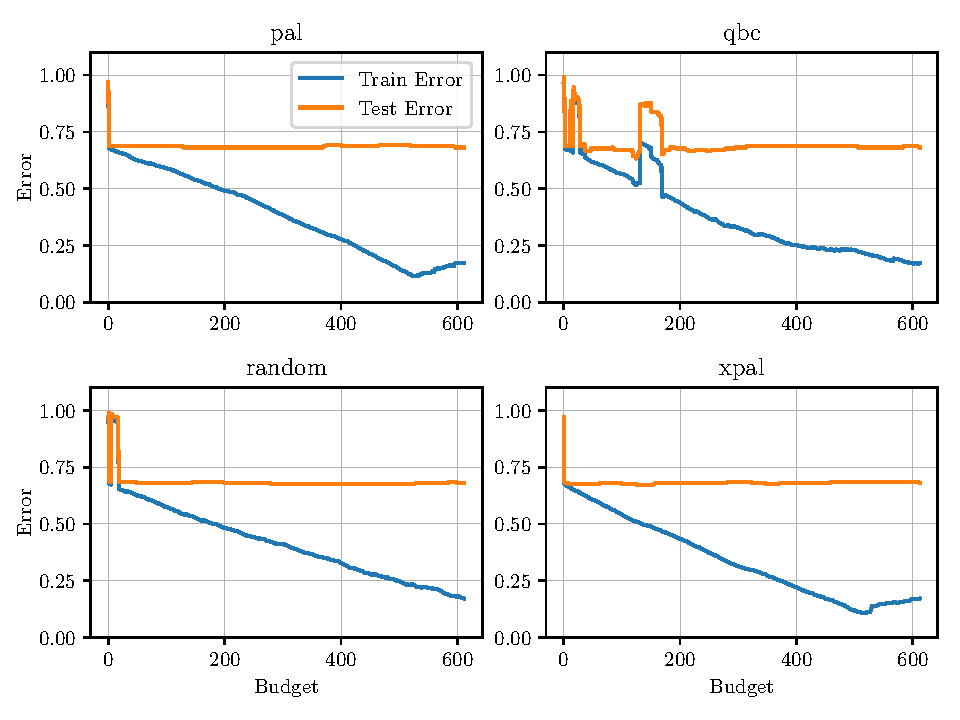
\includegraphics[width=\scale\textwidth]{../img/plot_all_results_rbf.pdf}
  \caption{Train and test error using different query strategies and RBF kernel for the PWC classifier.}
  \label{fig:plot_all_results_rbf}
\end{figure}

The radial bias function (RBF) kernel is a popular kernel function. It is defined as:

\begin{equation}
    K(x_i, x_j) = \exp\left(- \frac{\left\| x_i - x_j \right\|^2}{2 \sigma^2}\right)
\label{eq:rbf_kernel}
\end{equation}

where $\sigma$ is a parameter that controls the smoothness of the kernel and $x_i$ and $x_j$ are the two points in the feature space to compare. As seen in the Figure \ref{fig:plot_all_results_rbf} when the PWC classifier uses the RBF kernel it doesn't perform well with this data.

Starting with the data in Figure \ref{fig:plot_all_results_rbf} we made an error while constructing the $x$ dataset. While preparing the data, the TF-IDF vectorizer was fitted using all the data instead of just the training data. This resulted in the TF-IDF matrix having more information about the test data than it should have so our testing error results are likely lower than they should be. This error persists throughout the rest of the experiments in this chapter up until the experiments in Section \ref{sec:proper_vectorization}.

\subsection{Active Learning with PWC and Cosine Kernel}

In Figure \ref{fig:plot_all_results_cosine} we have the train and test errors for the same four different active learning sampling strategies tested on the same data. The only change was that we used Cosine kernel instead of the RBF kernel.The Cosine kernel is another important kernel function that is used in many machine learning algorithms. It is defined as:

\begin{equation}
    K(x_i, x_j) = \frac{x_i \cdot x_j}{\left\| x_i \right\| \left\| x_j \right\|}
\label{eq:cosine_kernel}
\end{equation}

where $x_i$ and $x_j$ are the two points in the feature space to compare. We found that using the Cosine kernel reduced the test error across the board by $\sim$15\%.  

\begin{figure}[ht]
  \centering
  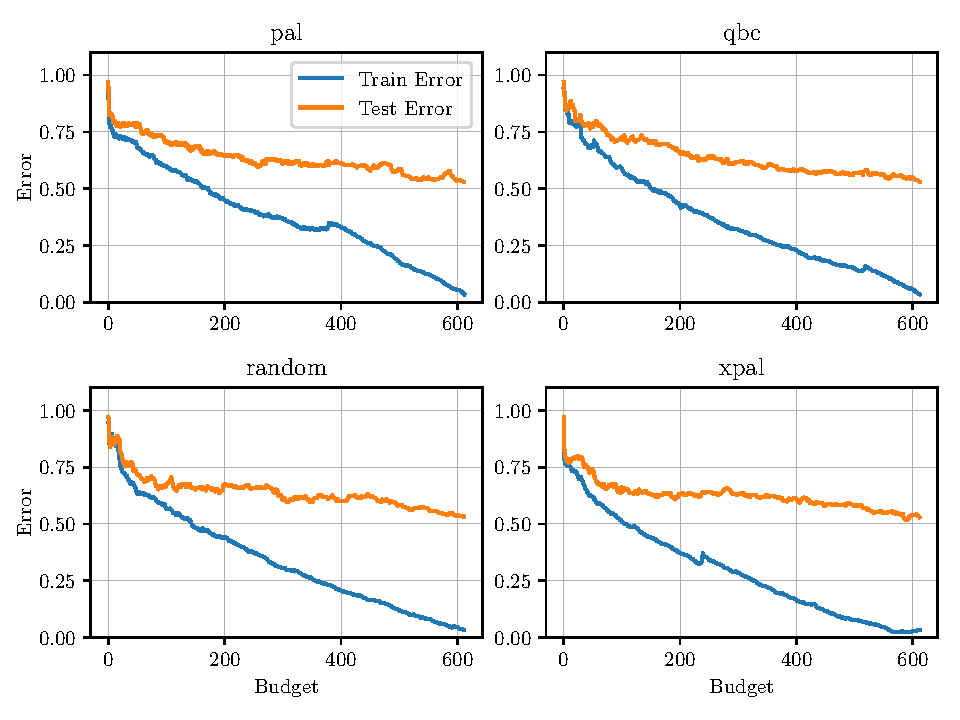
\includegraphics[width=\scale\textwidth]{../img/plot_all_results_cosine.pdf}
  \caption{Train and test error using different query strategies and Cosine kernel for the PWC classifier.}
  \label{fig:plot_all_results_cosine}
\end{figure}


In Figure \ref{fig:plot_all_results_cosine} PAL and xPAL were able to reduce the training error, by about 20\% and 25\% respectively, early in the training process compared to random selection and QBC. We also tested the other sampling strategies with the Cosine kernel and found that the results were similar. The other sampling strategies and their test data results are shown in Table \ref{fig:cos_test_results} along with the test data from Figure \ref{fig:plot_all_results_cosine}. 


\begin{figure}[ht]
    \centering
    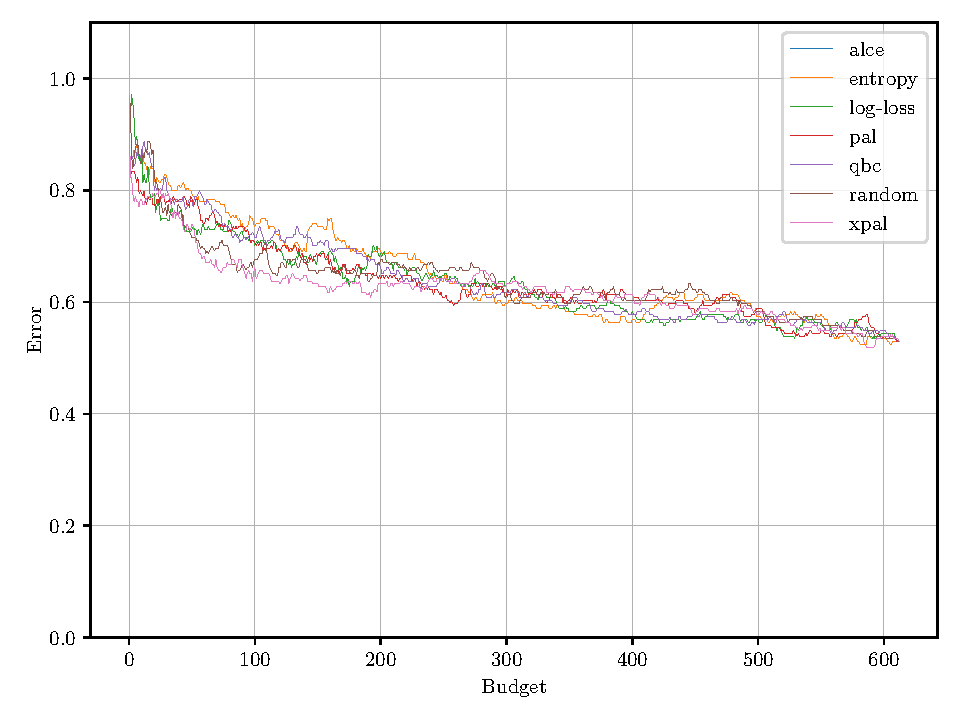
\includegraphics[width=\scale\textwidth]{../img/plot_kernel_cos_test_results.pdf}
    \caption{Comparing test error with one data split using different query strategies and Cosine kernel for the PWC classifier.}
    \label{fig:cos_test_results}
\end{figure}

We can see that the sampling strategies test performance converges over time (as we are using the same data and classifier) but xPAL appears to have an absolute minimum near the 600 budget mark in comparison to all sampling strategies. XPAL also appears to be performing well early on in the training process, in the 100-200 budget range. However, this test is only showing the results of one data split. We can get a better idea if we run more tests with different train-test splits and see how the results average out.

Figure \ref{fig:cos_test_results} shows that xPAL seems to be performing the best with our data but we wanted to see if we ran more tests with different train-test splits how the results would average out and which sampling strategy would perform the best on average. We ran 10 different data splits with each of the 7 sampling strategies and then took the average to get a smoother curve compared to the single run results shown in Figure \ref*{fig:cos_test_results}. The results for this experiment are shown in Figure \ref{fig:cos_avg_test_results}. 

It is clear in Figure \ref{fig:cos_avg_test_results} that xPAL is performing the best early on (budget from 0-100) in the sample selection process. XPAL selects the data that minimizes the test error and builds the strongest classifier quickly while it takes the other sampling strategies more data points to get to the same level of performance. Around the 100 budget mark we can see that the other selection strategies catch up to xPAL performance wise.

\begin{figure}[ht]
    \centering
    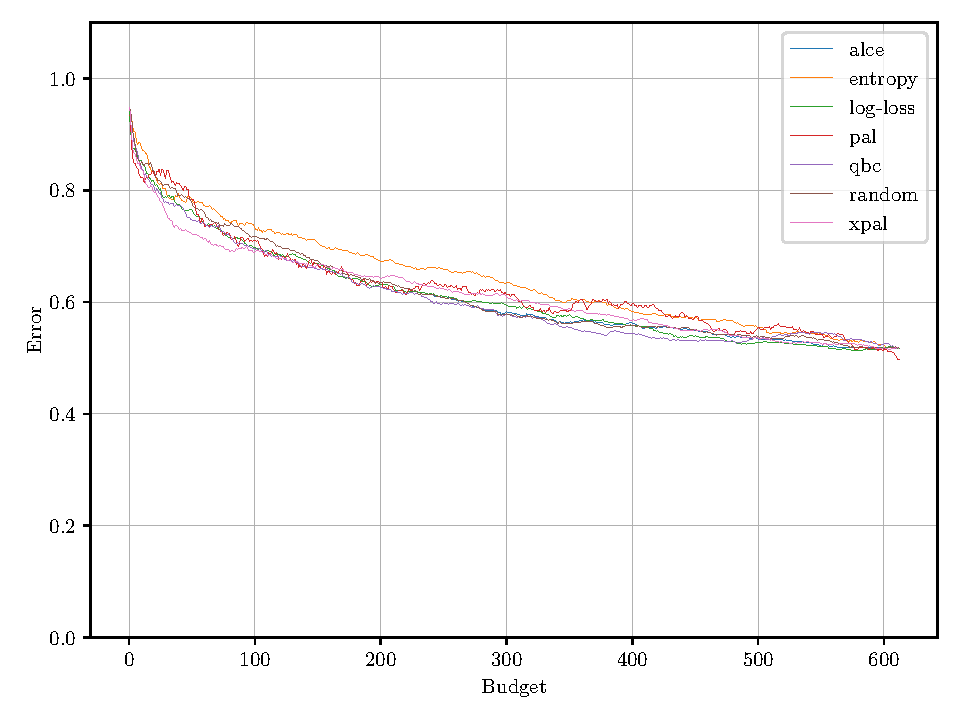
\includegraphics[width=\scale\textwidth]{../img/plot_kernel_cos_averaged_test_results.pdf}
    \caption{Comparing test error using different query strategies and Cosine kernel for the PWC classifier with results averaged over ten different data splits.}
    \label{fig:cos_avg_test_results}
\end{figure}


\subsection{Classifier Evaluation}

We also decided to test out some classifiers from the Scikit-Learn library to compare performances. Again we used the original data with the same TF-IDF vectorizer as used with the previous active learning models to stay consistent. It should be noted that cross validation was used here for evaluation but it was not used in the previous sections.

The goal of this exploratory phase was to try and decide which classifier to conduct more thorough testing with. As a result, we didn't use GridSearchCV for each classifier at this stage and we mostly used the default parameters and their cross validation scores with all of the original data (i.e. additional data not included). In some cases where using weights was an option for the classifier we included the precomputed Cosine decay weights. A table of the parameters used for each classifier is shown in Appendix Table \ref{tab:explore_classifiers_params}.

Initially we made a minor error while evaluating the classifiers that used the precomputed weights in the following experiments. While computing the accuracy scores for the classifiers, we failed to incorporate the class weights that were used in training the classifier. This resulted in the accuracy scores being incorrectly calculated. This error persists throughout the rest of the experiments in this chapter up until the experiments in Section \ref{sec:proper_vectorization}.

The results for the different classifiers are shown in Figure \ref{fig:explore_classifiers}. In the box-plot, the whiskers extend from the box to the furthest data points that are within 1.5 times the inter-quartile range (IQR) of the box. Any data points that are beyond the whiskers are considered outliers and are plotted as individual points or symbols (diamonds) as seen in the figure.


\begin{figure}[ht]
  \centering
  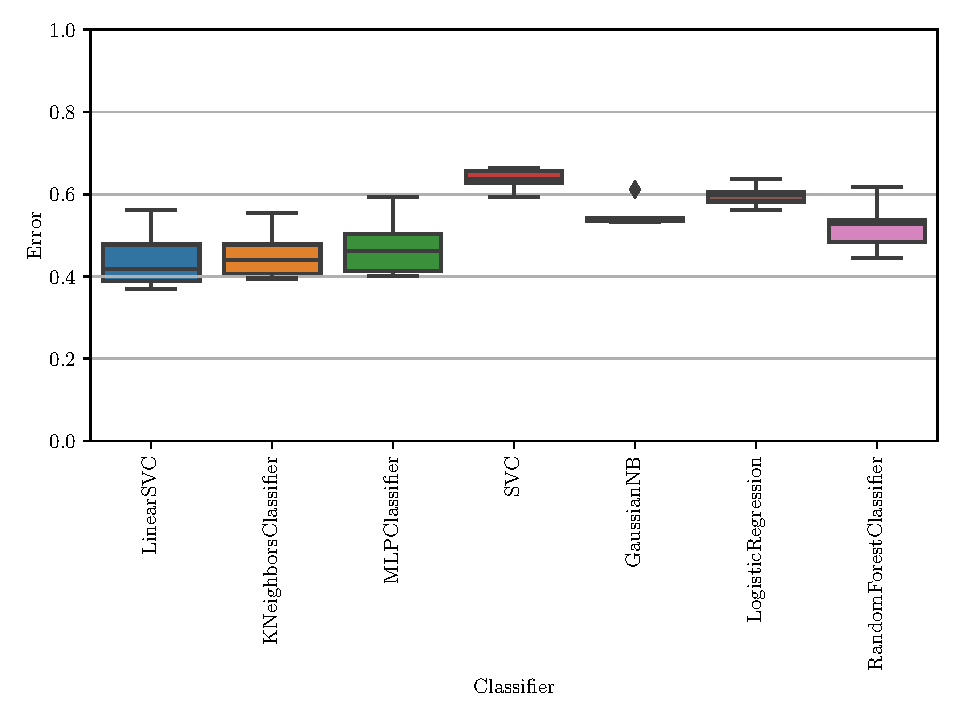
\includegraphics[width=\scale\textwidth]{../img/plot_explore_classifiers.pdf}
  \caption{Performance of classifiers without GridSearchCV optimization.}
  \label{fig:explore_classifiers}
\end{figure} 

The base LinearSVC classifier model performed best compared to other classifiers and it is a fast running algorithm even with data that has many features. We decided to look further into LinearSVC because it performed so well. We also wanted to conduct more testing with KNeighborsClassifier and Neural Networks. 

We created three models for LinearSVC, the first was a boilerplate LinearSVC with no argument modifications, the second model used the class weights parameter set to 'balanced'. The 'balanced' mode uses the values of y to automatically adjust weights inversely proportional to class frequencies in the input data as $n\_samples / (n\_classes * np.bincount(y))$. 

For the third test we created a dictionary of weights for each class using the Cosine decay function. The weights for each category ranged from 0.1 to 1.0 where the most frequent classes had smaller weights. The Cosine decay function is defined as:

\begin{equation}
    w_i = \frac{1}{2} \left(1 + \cos \left(\frac{\pi t}{T}\right)\right)
\label{eq:cosine_decay}
\end{equation}

where $w_i$ is the weight for the $i^{th}$ class, $t$ is the current iteration, and $T$ is the total number of iterations. The Cosine decay function is a common function used for weights in machine learning algorithms. The calculated cosine weights are shown in the appendix in Table \ref{tab:cosine_decay_weights}.

The results for the LinearSVC classifier experiments are shown in Table \ref{tab:lsvc_errors} where the LinearSVC with the Cosine decay weights didn't perform better than the other LinearSVC models.

\begin{table}[!ht]
\centering
\caption{Error for three differing LinearSVC models.}
\begin{tabular}{lr}
\toprule
               Model &  Error \\
\midrule
Cosine Decay Weights &  0.392 \\
         Boilerplate &  0.407 \\
    Balanced Weights &  0.441 \\
\bottomrule
\end{tabular}

\label{tab:lsvc_errors}
\end{table}

Using K-Neighbors Classifier (KNN) and a Neural Network from TensorFlow we conducted additional experiments. For the KNN we found that using 8 neighbors and the cosine distance metric provided the lowest error. 

For the Neural Network we used a dense hidden-layer with 1000 neurons with Sigmoid activation and 23 output neurons with Softmax activation. For the NN optimizer we used Adamax with Cosine decay with an initial learning rate of 0.1, alpha value of 0.1 and 915 decay steps ($X\_data\_size // batch\_size * num_epochs$). The results are shown in Table \ref{tab:best_errors}. We can see that the K-Nearest Neighbors classifier and the Neural Network classifier performed slightly worse compared to LinearSVC.

The LinearSVC outperformed the other classifiers and we decided to experiment with it further. We attempted to boost performance of the LinearSVC classifier using multiple cross validation grid searches with the bagging. Bagging (bootstrap aggregating) is a type of ensemble learning, where multiple models are trained on different subsets of the training data and their predictions are combined to make the final prediction. In Scikit-Learn we used the BaggingClassifier to implement bagging. An example of our setup and parameters are shown in the code snippet. 

\begin{lstlisting}[language=Python]
base_classifier = LinearSVC()
bagging_classifier = BaggingClassifier(
    base_estimator = base_classifier,
    n_estimators = 20, 
    random_state = args.seed)
params = {
    'base_estimator__random_state': [args.seed],
    'base_estimator__max_iter': [10000],
    'base_estimator__intercept_scaling': 
        np.linspace(0.1, 1, 20),
    'base_estimator__loss': ['hinge', 'squared_hinge'],
    'base_estimator__penalty': ['l1', 'l2'],
    'base_estimator__class_weight': [None, weights],
    'base_estimator__C': np.linspace(0.1, 1000, 50),
    'base_estimator__multi_class': ['ovr', 
        'crammer_singer']
    }
\end{lstlisting}

Performance was not improved from what we had already seen. Using bagging may not be the best approach at this stage because there are some categories that have very few samples so bagging may be unable to create a good model. We will revisit bagging in future chapters when we have more data at our disposal. We also didn't use the balanced class weights parameter because we had already seen that it was the worst performing class weight parameter in previous tests. The BaggingClassifier and GridSearchCV combination didn't improve the performance of the LinearSVC classifier beyond what we had already achieved.

\begin{table}[h]
\centering
\caption{Testing errors for best performing classifiers.}
\begin{tabular}{lr}
\toprule
         Model &  Error \\
\midrule
     LinearSVC &  0.392 \\
Neural Network &  0.446 \\
           KNN &  0.451 \\
\bottomrule
\end{tabular}

\label{tab:best_errors}
\end{table}

The precision-recall curve for the best performing classifier (LinearSVC) is shown in Figure \ref{fig:pr_curve} and the confusion matrix is shown in Figure \ref{fig:confusion_matrix} for the best performing LinearSVC classifier.The precision-recall curve gives us an idea at how well our classifier can correctly categorize the data. It also gives us a visualization of how unbalanced our categories are. We can see this imbalance clearly in Figure \ref{fig:pr_curve} where we have straight lines and large steps for some categories. This is a result of having a small number of data in a class. However, we can also see that for some classes the precision is relatively high even though we have few data points. Here we are namely concerned with the 'Culture' and 'Beauty' categories which have 10 and 31 data points respectively. It may be that the keywords in the 'Culture' and 'Beauty' categories are drastically different from the other categories so the performance is better. 

\begin{figure}[h]
  \centering
  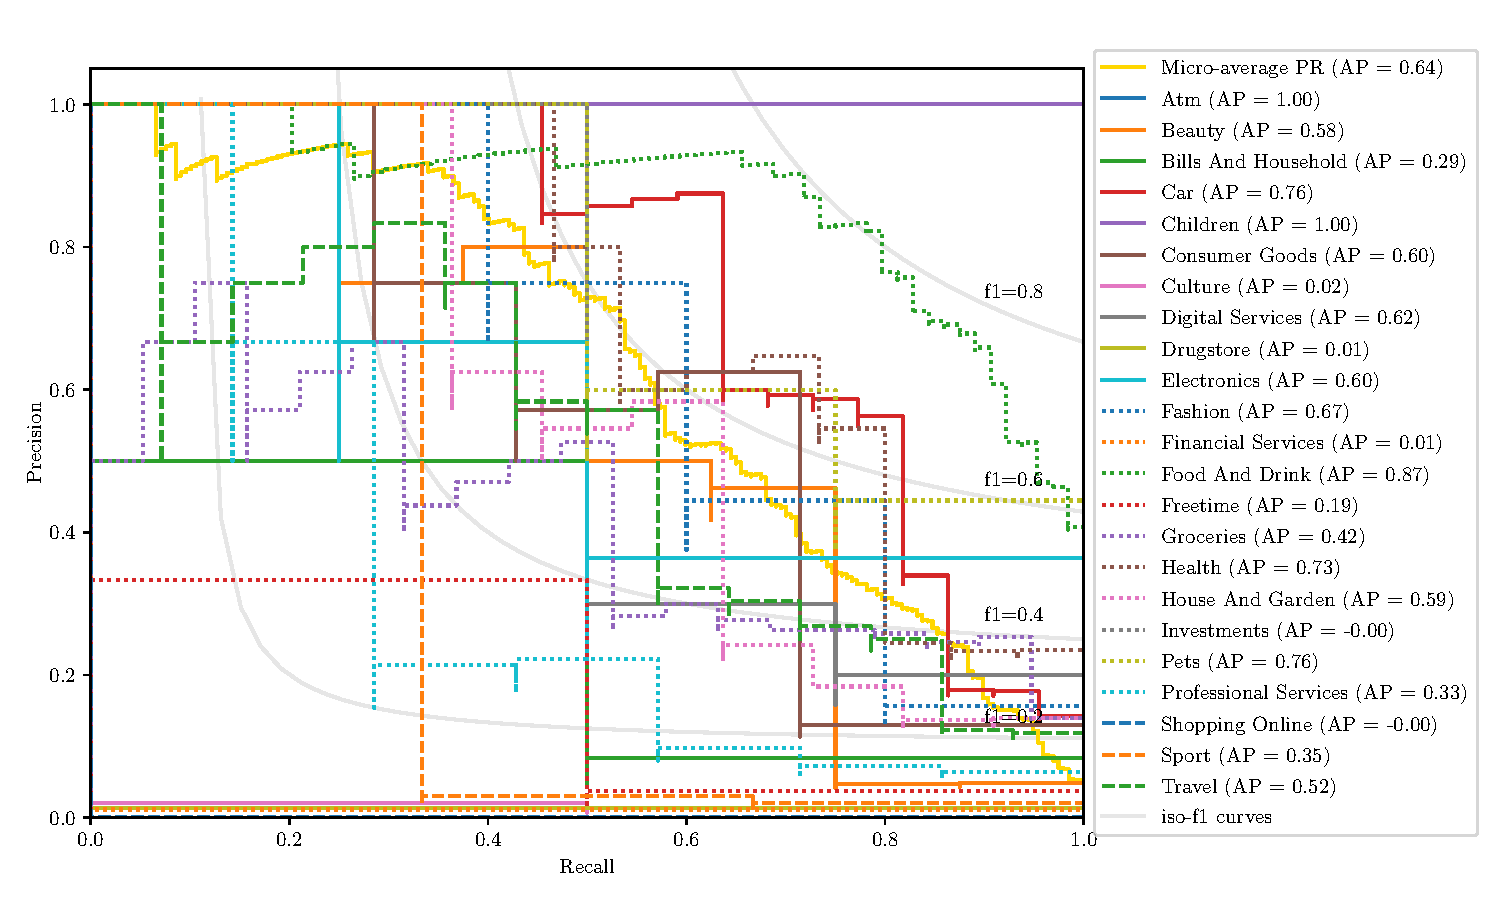
\includegraphics[width=\scale\textwidth]{../img/plot_pr_curve.pdf}
  \caption{Precision-recall curve for the best performing LinearSVC classifier.}
  \label{fig:pr_curve}
\end{figure}

The confusion matrix shown in Figure \ref{fig:confusion_matrix} may be a better metric for visualizing this data. In addition, the classification report for the LinearSVC classifier is shown in Appendix Table \ref{tab:classification_report_LinearSVC} with F1, accuracy, precision, recall, and support scores.

\begin{figure}[h]
  \centering
  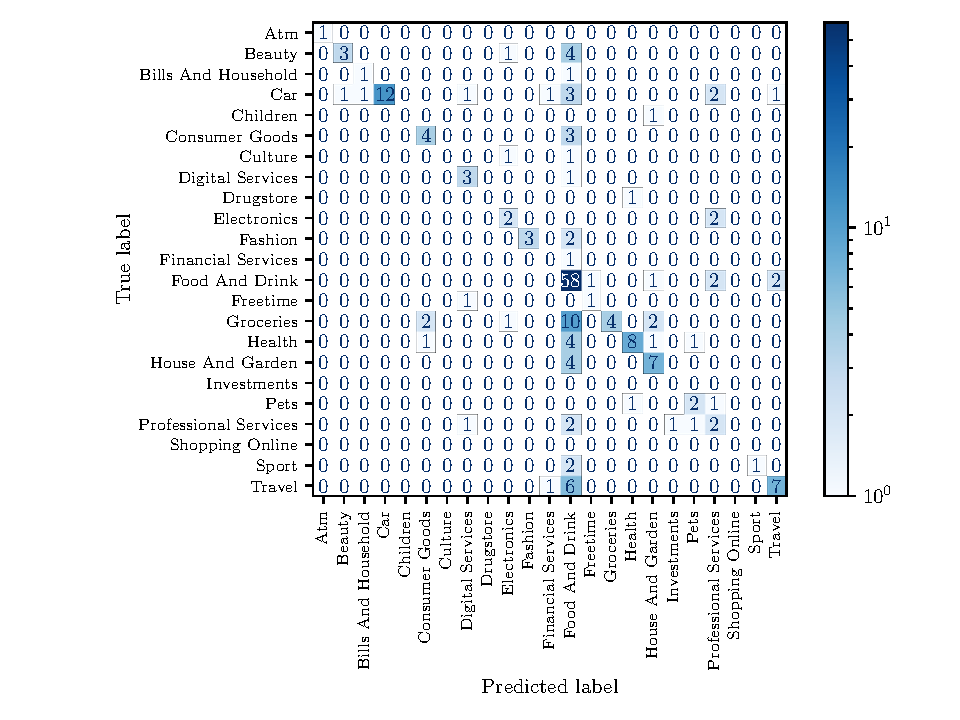
\includegraphics[width=\scale\textwidth]{../img/plot_cm_LinearSVC.pdf}
  \caption{Confusion matrix for the best performing LinearSVC classifier using the original data.}
  \label{fig:confusion_matrix}
\end{figure}


\section{All Data}
\label{sec:proper_vectorization}

In this section we will take what we have learned from the experiments in the previous sections and apply that knowledge to the original data set augmented with the additional data that we collected. This will provide us with a better understanding of how the data is interacting with the active learning sampling strategies and the PWC classifier. We will also removing some data from the set if the text length is below some threshold, evaluate the performance with a reduced number of categories, and explore the performance of xPAL with using all available data.

\subsection{Active Learning with Additional Data}

In this experiment we tested all the active learning methods with the corrected TF-IDF vectorizer transformation. In this section instead of incorrectly vectorizing the data then importing it to be used with \cite{kottke2021toward} probablistic active learning code, we exported the raw text data and then split the text data, fit and transformed the vectorizer to the train data, then transformed the test data and conducted our experiments with the modified code.

We then used the different active learning methods and PWC with the Cosine kernel to run our experiments. We ran 10 test runs for each method and then averaged the test error of all the runs resulting in a single curve for each sampling strategy. We only used the first 300 data points instead of using all available data. As a result, the test error doesn't converge in this plot because we are only using a subset of the data. The results are shown in Figure \ref{fig:active_learning_new_data_new_vect}.

\begin{figure}[h]
  \centering
  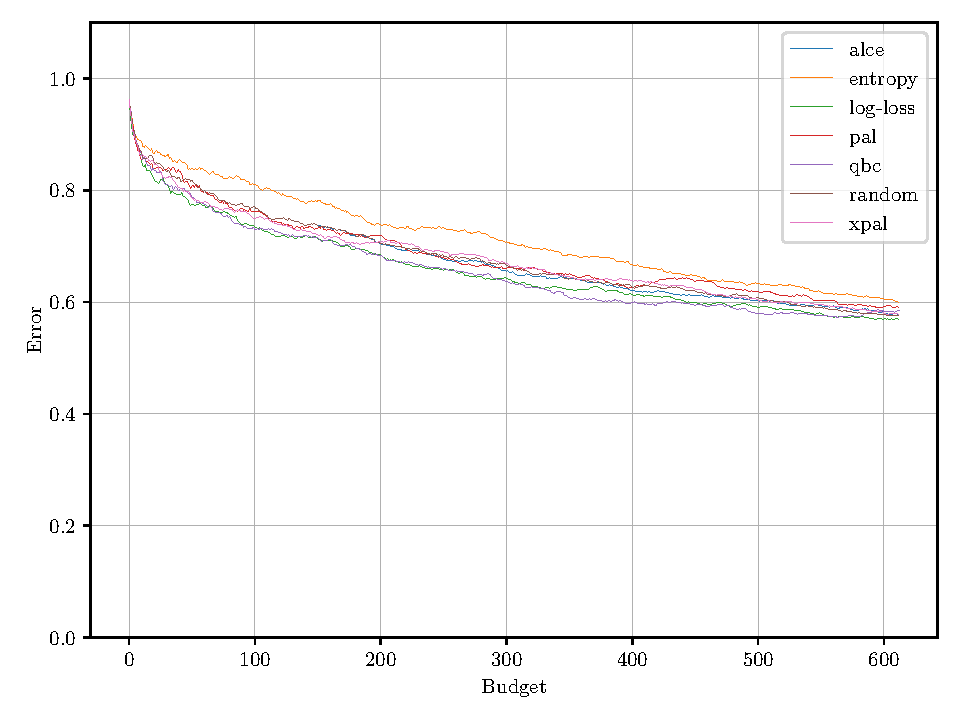
\includegraphics[width=\scale\textwidth]{../img/plot_all_data_new_vectorizer_test_results.pdf}
  \caption{Active learning results with using all data.}
  \label{fig:active_learning_new_data_new_vect}
\end{figure}

Its clear that active learning sampling strategies found it more difficult with this additional data compared to our previous runs. We can clearly see that the xpal-original outperformed all other sampling strategies.

When making more data available to the classifier we assumed that the test error would decrease. However, it may be the case that the additional data is not as useful as we thought.

\subsection{LinearSVC with Additional Data}

We have some data that may not have enough text to classify correctly and others that have more than 1000 characters of text that may be noisy. We also know that sometimes while scraping the text data from a website we collected a non empty string that in reality provided no words that were related to the label.

However, using all available data, we now have the luxury of having more than the minimum of 2 data points in some categories and can afford to remove data from the set that may only have two or three strings in the text. We decided to explore if filtering the data based on text length could improve the performance of the classifier and use LinearSVC as it has performed well with this data previously and it is relatively fast to train.

We imported the data and either selected a minimum number of characters or we altered the maximum number of characters allowed and created a new dataset. For each run we selected the data based on this criteria and then built the TF-IDF array. For the minimum string size tests we incremented the string size by 1 character. While for the max string size tests we decremented the string size by 10. We again used a train test split of 25\% which has been our standard for testing throughout our experiments. We found that around the 200 character mark we would filter out too much data and would not have a minimum representation (2 data points) for all the categories. The results for this experiment are shown in Figure \ref{fig:grid_search_text_length}.

\begin{figure}[h]
    \centering
    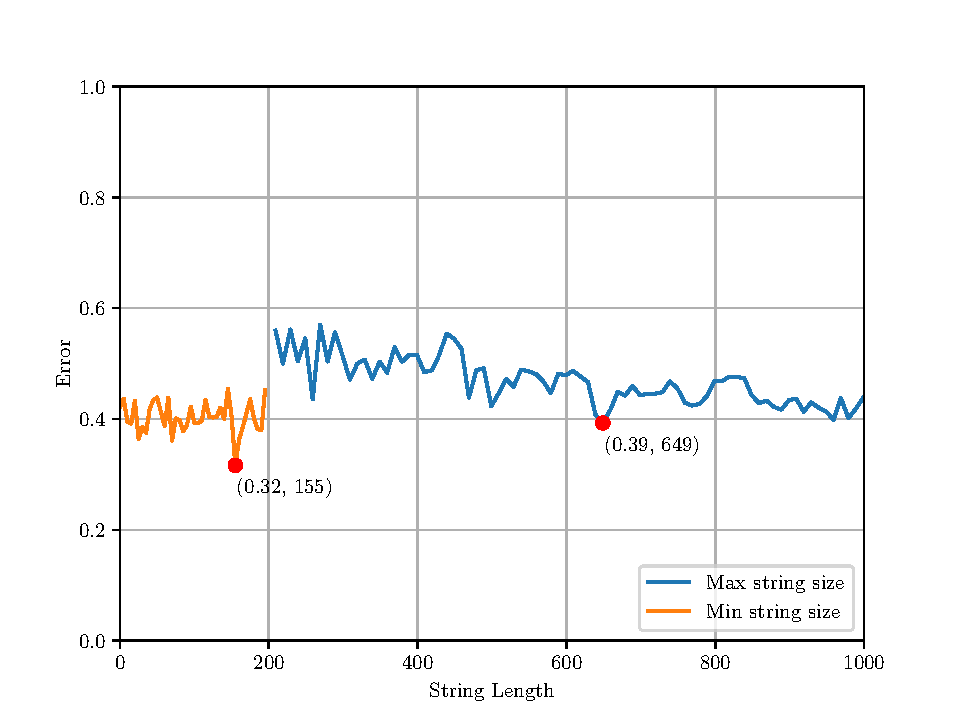
\includegraphics[width=\scale\textwidth]{../img/plot_data_length_grid_search.pdf}
    \caption{Test error results for best LinearSVC with varying text length parameters.}
    \label{fig:grid_search_text_length}
  \end{figure}

We also tested with a minimum text length and a maximum text length constraint implemented together but this combination did not yield any obvious gains.

This naive approach to filtering the data did not yield any obvious improvements in the test error. At best it may have filtered out some bad data and provided a small improvement in the test error. However, when implementing xPAL we hope to have it filter out the bad data in a more calculated manner.

% \begin{figure}[ht]
%     \centering
%     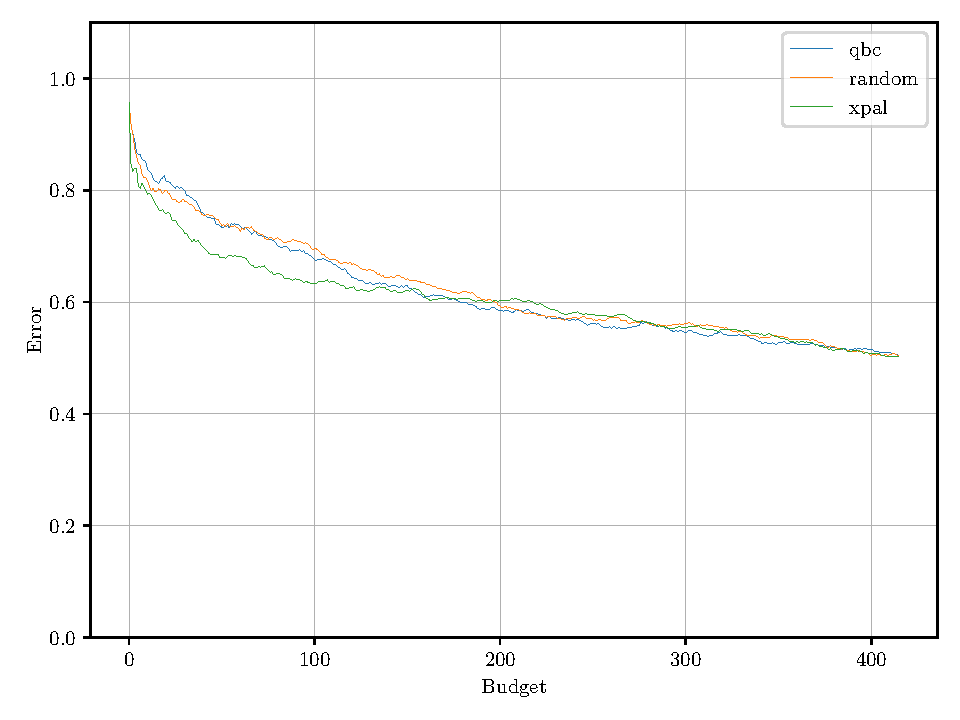
\includegraphics[width=\scale\textwidth]{../img/plot_filtered_test_results.pdf}
%     \caption{Test error results using filtered data with minimum 155 character length with PWC and Cosine kernel.}
%     \label{fig:probal_filtered_data}
%   \end{figure}

We can see that for the 414 data points results from the filtered data in the train split converge as we expect to a single point because the PWC has access to all of the labeled train data. 

\subsection{Active Learning Revisited}

With the new filtered data set we also wanted to see how the PWC classifier with active learning would perform. We used the same text length constraints as mentioned in the previous section and evaluated the data with the PWC classifier with the Cosine kernel. 

We chose to test with the QBC selection strategy in addition to xPAL because QBC appeared to perform well in previous tests and it is much faster to calculate in comparison to PAL. The results show that the PWC was able to make some small improvements in the test error overall but also that the new data allowed the xPAL selection strategy to decrease the test error even more rapidly than before when we used the original data, and it took less data.

TALK ABOUT DISTRIBUTION USING ORIFINAL AND ALL DATA INSERT PLOT HERE 

\subsection{Active Learning with Less Categories}

\chapter{Testing with All Data}
\label{sec:proper_vectorization}

In this section we will take what we have learned from the experiments in the previous sections and apply that knowledge to the original data set augmented with the additional data that we collected (i.e all data or all useable data). The total category count tallies can be located in the Attachments in Table \ref{tab:data_counts}. We hope these experiments will provide us with a better understanding of how the data is interacting with the active learning sampling strategies and the PWC classifier. We will also try removing some data from the set if the text length is below some threshold, and evaluate the performance with a reduced number of categories.

\section{Classifier Evaluation Revisited}

We wanted to re-run the classifier experiment that we ran with the original data with the new data to get an idea of how the new data performed with the classifiers from Scikit-Learn. The results are shown in Table \ref{tab:best_errors_all_data}.

\begin{table}[ht]
    \centering
    \caption{Test errors for best performing classifiers using all data.}
    \begin{tabular}{lr}
\toprule
                     Model &  Error \\
\midrule
                 LinearSVC &  0.429 \\
Tensor Flow Neural Network &  0.433 \\
    K Neighbors Classifier &  0.471 \\
\bottomrule
\end{tabular}

    \label{tab:best_errors_all_data}
\end{table}

Its interesting to see that the errors increased across the board but our previous results could have been skewed possibly because we had so few data samples in some categories. We ran the Bagging Classifier GridSearchCV from the previous chapter and again could not tune the model to perform better than the base untuned LinearSVC.

\section{Active Learning using All Data}

In these experiments we tested all the active learning methods available in the repository from the paper by \cite{kottke2021toward}. We encoded all available text data using TF-IDF as we had done previously. In Figure \ref{fig:probal_original_proper_vect} we show a previous experiment using just the original data so we could have a more accurate comparison with the results for all the data shown in Figure \ref{fig:probal_all_proper_vect}. In Figures \ref{fig:probal_original_proper_vect_50_st_filter} and \ref{fig:probal_all_proper_vect_50_st_filter} we used an arbitrary text length filter of 50 characters to see how the performance of the selection strategies changed when we removed some of the data. The categorical data splits for the 50 character filter can be found in the Attachments in Table \ref{tab:50_char_filter_data_counts}.

\begin{figure}[ht]
    \centering
    \begin{subfigure}{0.49\textwidth}
        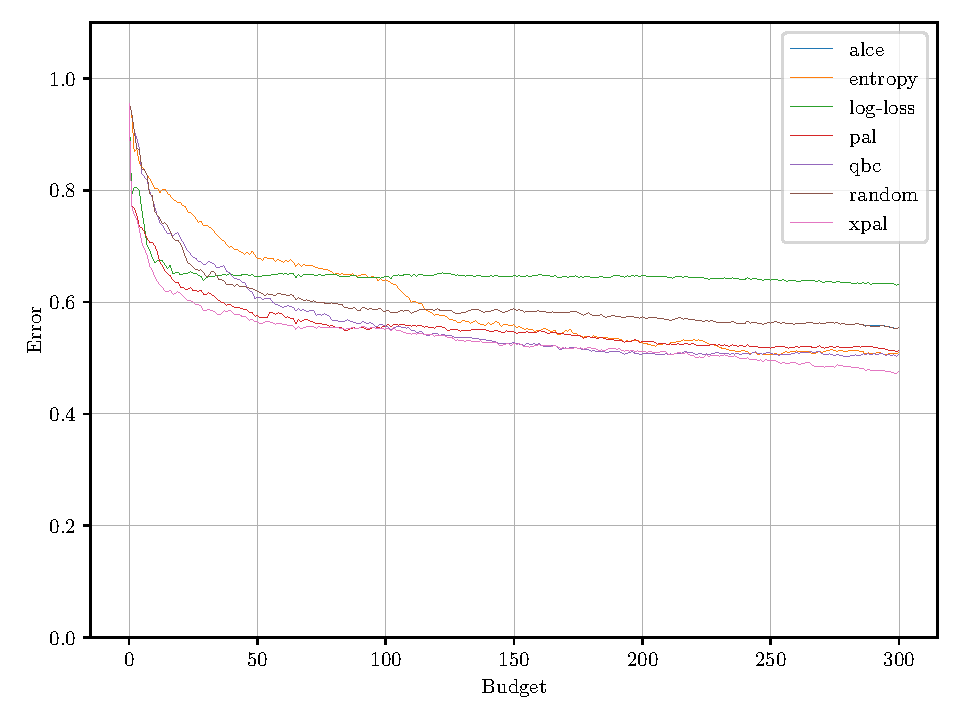
\includegraphics[width=\textwidth]{../img/plot_text_data_original_proper_vectorizer_test_results}
        \caption{No text length filter.}
        \label{fig:probal_original_proper_vect}
    \end{subfigure}
    \hfill
    \begin{subfigure}{0.49\textwidth}
        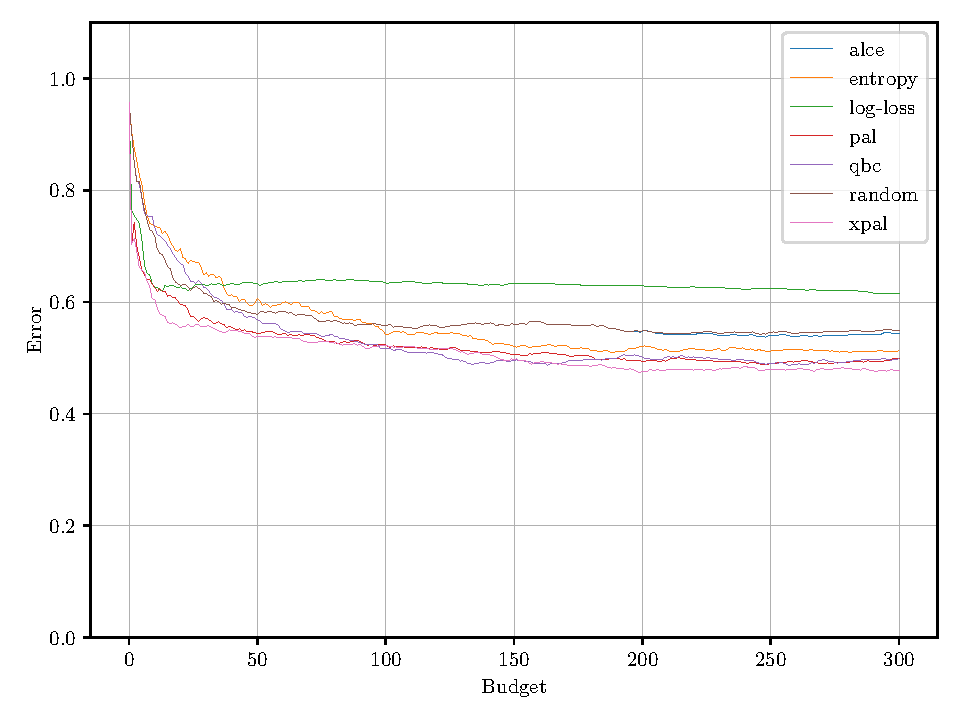
\includegraphics[width=\textwidth]{../img/plot_text_data_original_proper_vectorizer_50_st_filter_test_results}
        \caption{Text length data $>50$.}
        \label{fig:probal_original_proper_vect_50_st_filter}
    \end{subfigure}
    \caption{Active learning results using the original data.}
\end{figure}

We again used the different active learning methods and PWC with the Cosine kernel to run our experiments. We ran 10 test runs for each method and then averaged the test error of all the runs resulting in a single curve for each sampling strategy. We only used the first 300 data points instead of using the entire budget because we want to reduce the amount of time it takes to run our experiments. As a result, the test error doesn't converge in these plots. With the original data we can see that the xPAL sampling strategy finds the best data early (20-30 budget range) in the sampling process and exploits this to improve the classifier the most. Eventually we see that PAL and QBC have similar performance to xPAL but, ultimately, after 300 samples xPAL is the best performing sampling strategy. We also want to note that in \ref{fig:probal_original_proper_vect} the results for ALCE are almost entirely hidden behind the random sampling strategy curve. 

Using all the data, we repeated this same experiment. The results are shown in Figure \ref{fig:probal_all_proper_vect}. In both experiments in this section it appeared that the test error for xPAL was converging to around roughly 50\%. But for the second experiment using all the data xPAL was finding and exploiting the best data earlier and for longer in the sampling process. We can see the dominance of xPAL throughout the plot except around the 200 budget range where entropy sampling starts to momentarily perform well.

\begin{figure}[ht]
    \centering
    \begin{subfigure}{0.49\textwidth}
        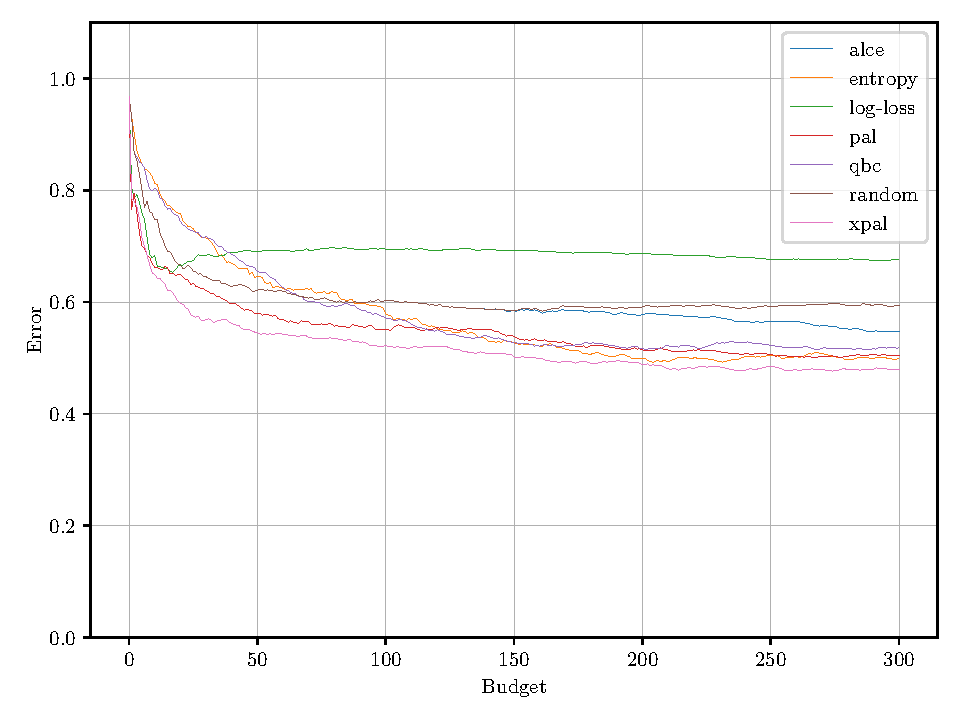
\includegraphics[width=\textwidth]{../img/plot_text_data_all_proper_vectorizer_test_results}
        \caption{No text length filter.}
        \label{fig:probal_all_proper_vect}
    \end{subfigure}
    \hfill
    \begin{subfigure}{0.49\textwidth}
        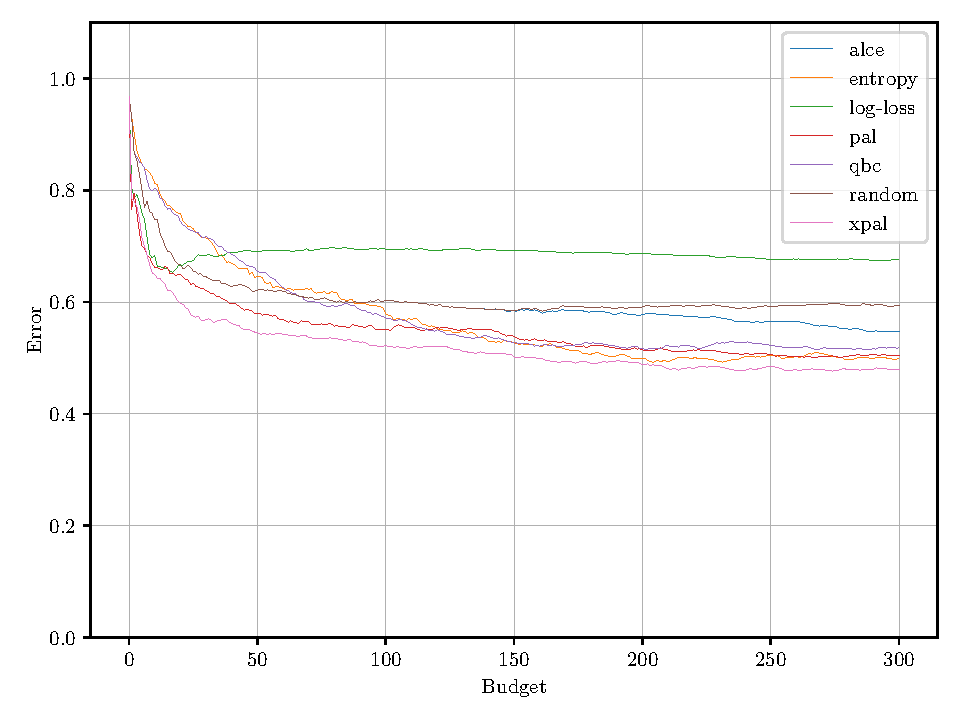
\includegraphics[width=\textwidth]{../img/plot_text_data_all_proper_vectorizer_50_st_filter_test_results}
        \caption{Text length data $>50$.}
        \label{fig:probal_all_proper_vect_50_st_filter}
    \end{subfigure}
    \caption{Active learning results using all data.}
\end{figure}

In both the re-run original data and all data experiments, xPAL appears to perform well on average over 10 different runs in comparison to the other selection strategies, it even seemed to perform markedly well with more data available and then having some filtering applied as shown in Figure \ref{fig:probal_all_proper_vect_50_st_filter} where it seemed to have some dominance over the other selection strategies. This led us to believe that the more data that is available and the more text that is available per data sample the better xPAL will perform. This will not always be true but it seems that if we have a large enough amount of text, 50 characters being an arbitrary example, xPAL will have an easier time selecting the best data points to label.

We were curious what xPAL was doing when more data was available, so while running the experiments we recorded when a data point was selected (its index in the selection budget) and for which category it was selected from. This data is shown in Figure \ref{fig:xpal_data_selection}.

\begin{figure}[ht]
  \centering
  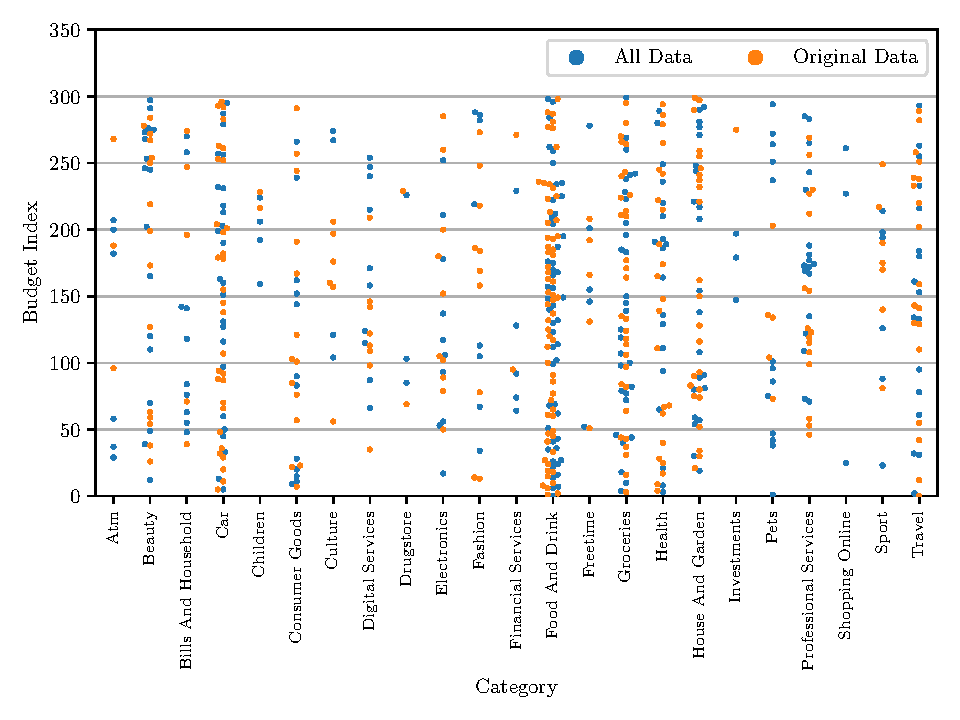
\includegraphics[width=\textwidth]{../img/plot_xpal_selection_dist}
  \caption{Data point selection swarm plot using xPAL.}
  \label{fig:xpal_data_selection}
\end{figure}

This distribution data is from a sample run for each of the data sets without any filtering. In this data split the 'Shopping Online' category for the original data went without asking for a label in the given budget window. It is interesting that it chose not to select its sole sample but, intuitively, it may make sense because there is only one other 'Shopping Online' sample point and it is in the test set. Its possible that because there is only one sample xPAL may not yet find it necessary to know its label this early in the budget and other data points labels are more valuable to know. It is clear from Figure \ref{fig:xpal_data_selection} that when new data is available the xPAL selection strategy reevaluates what is important and selects data points that are more likely to be helpful. This is a good sign that xPAL is able to adapt to the data and find the most helpful data points.

\section{LinearSVC with Text Length Filtering} 

We have some data that may not have enough text to classify correctly and others that have more than 1000 characters of text that may be noisy. We also know that sometimes while scraping the text data from a website we collected a non empty string that actually provided no words that were related to the label, such as a simple error or warning message.

Using all available data, we now have the luxury of having more than the minimum of 2 data points in some categories and can afford to remove data from the set that may have unhelpful or confusing words. We decided to explore if filtering the data based on text length could improve the performance of the classifier and use LinearSVC as it has performed well with this data previously and it is relatively fast to train.

Before conducting the filtering data experiments we can view how the text length is distributed throughout our text data as shown in Figure \ref{fig:string_length_dist}. This helps us visualize how much data we may be removing if we filter the data based on text length.

\begin{figure}[ht]
    \centering
    \begin{subfigure}{0.49\textwidth}
        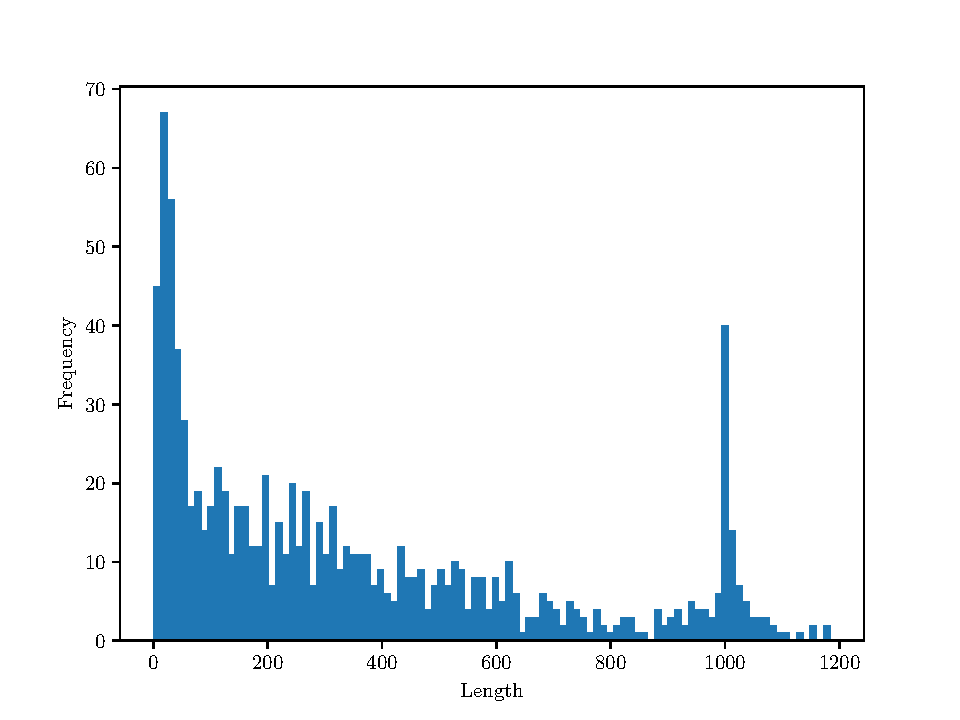
\includegraphics[width=\textwidth]{../img/plot_string_length_dist_all_data}
        \caption{Distribution of text length for all data in 100 bins.}
        \label{fig:string_length_dist}
    \end{subfigure}
    \hfill
    \begin{subfigure}{0.49\textwidth}
        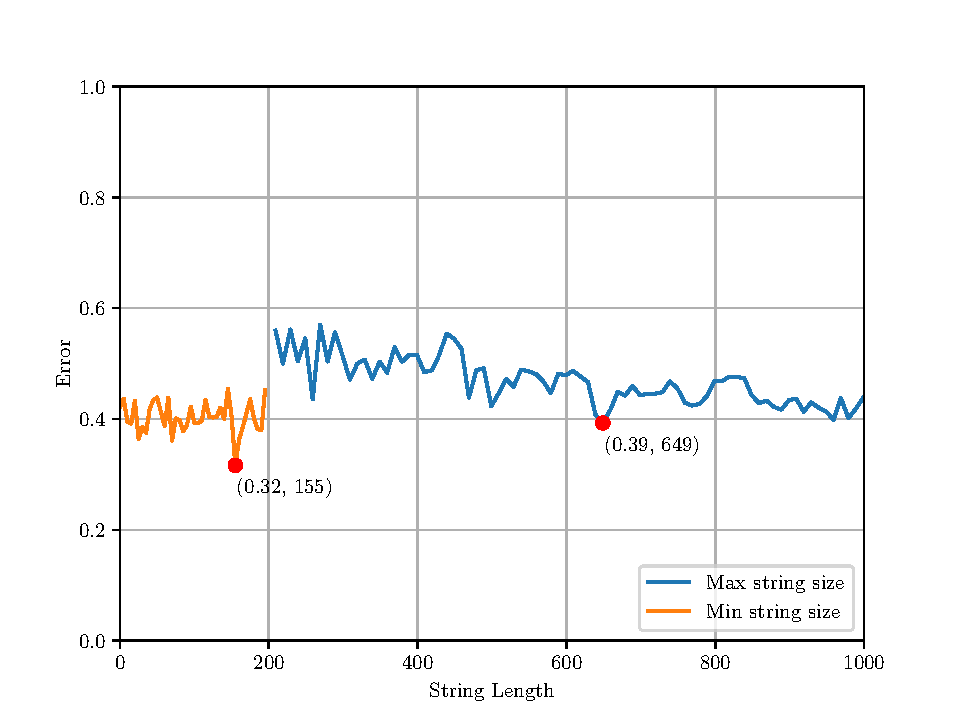
\includegraphics[width=\textwidth]{../img/plot_data_length_grid_search}
        \caption{Test error results for best LinearSVC with varying text length requirements.}
        \label{fig:grid_search_text_length}
    \end{subfigure}
    \caption{Text length experiments data and results.}
\end{figure}

The distribution of the text show a steady decrease in length and frequency until around the 1000 length mark where we have an increase of data with large amounts of text. The spike here is a results from when we capped the non English data text to 1000 characters so that we could translate all of our data using the Azure translation services.

We imported the data and either selected a minimum number of characters or we altered the maximum number of characters allowed and created a new dataset. For each run we selected the data based on this criteria and then built the TF-IDF array. For the minimum string size tests we incremented the string size by 1 character. While for the max string size tests we decremented the string size by 10. We again used a train test split of 25\% which has been our standard for testing throughout our experiments. We found that around the 200 character mark we would filter out too much data and would not have a minimum representation (2 data points) for all the categories. The results for this experiment are shown in Figure \ref{fig:grid_search_text_length}.

We also tested with a minimum text length and a maximum text length constraint implemented together but this combination did not yield any obvious gains. This naive approach to filtering the data did not yield any obvious improvements in the test error. At best it may have filtered out some bad data and provided a small improvement in the test error. However, when implementing xPAL we hope to have it filter out the bad data in a more calculated manner.

\section{Testing with Fewer Categories}

In this section we will briefly look at the PWC with xPAL and LinearSVC performance using progressively fewer categories. We will use all available data and remove the category from the data set if it has less than the minimum number of samples. We assume that reducing the number of categories decreases the test error. Intuitively, this should be the case because as we reduce the number of categories we are reducing the number of classes that the classifier has to learn and classify. This should make the classification task easier and therefore the test error should decrease. However, we have a lot of data in the 'Food and Drink' and 'Groceries' categories and we have seen that the classifiers struggle to classify these categories correctly. Results from some tests are shown for the PWC with xPAL in Figure \ref{fig:all_data_category_reduction_xpal}.

\begin{figure}[ht]
    \centering
    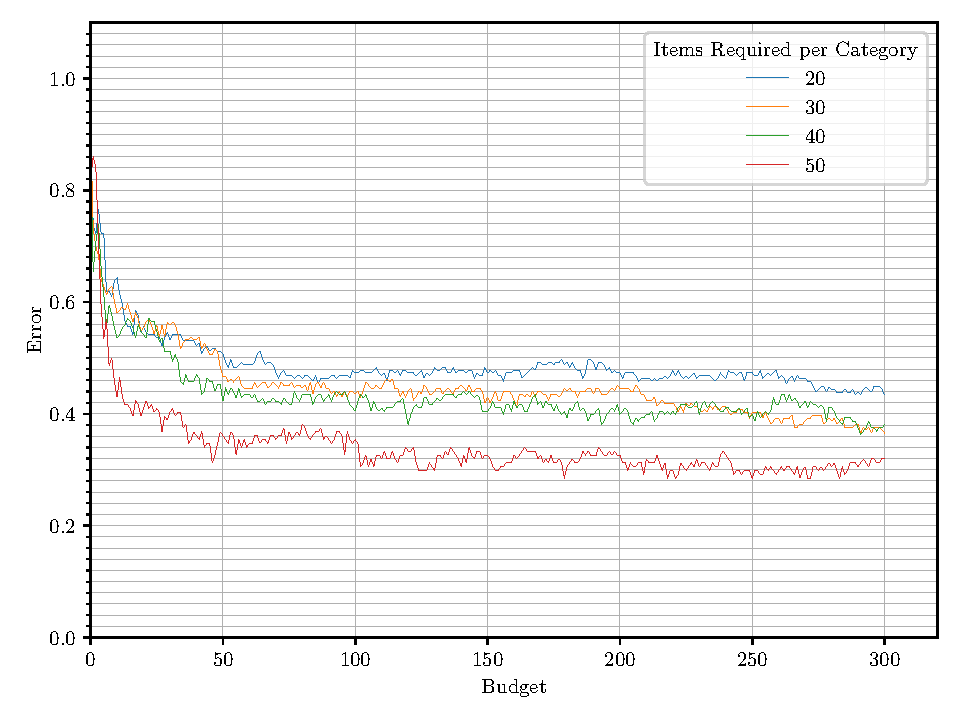
\includegraphics[width=\textwidth]{../img/plot_text_data_all_category_reduction_test_results}
    \caption{PWC with xPAL with category reduction on all data.}
    \label{fig:all_data_category_reduction_xpal}
\end{figure}

\cite{dumais2000hierarchical} discuss the issue of reducing the number of categories in web content classification in their paper. They note that reducing the number of categories can improve the accuracy and efficiency of the model by reducing the complexity of the classification problem. However, they also note that reducing the number of categories can reduce the specificity of the classification and make it more difficult to distinguish between similar categories.

Looking at the results from the xPAL and PWC tests in Figure \ref{fig:all_data_category_reduction_xpal} we can see that we have generally have reduction in test error except between the 30 and 40 category minimum tests. This table also shows us the categories that were used in the classification. This might tell us that 'Consumer Goods', 'House and Garden', and 'Professional Services' are easily linearly as the change in test error after 300 samples was small.

Reviewing these results it seems that 'Food and Drink' and 'Groceries' may be skewing a portion of the test error and if there was better way to classify these categories it would improve the overall test error.

\begin{table}[ht]
     \centering  
     \caption{LinearSVC performance with category reduction on all data, where category minimum is the min number of samples required.}
     \begin{tabular}{p{2cm}|p{1.8cm}|p{7.5cm}|p{1.4cm}}
\toprule
 Category Minimum &    Error &                                                                                                                              Categories &  Count \\
\midrule
               20 & 0.359756 & [Beauty, Car, Consumer Goods, Fashion, Food And Drink, Groceries, Health, House And Garden, Pets, Professional Services, Sport, Travel] &     12 \\
               30 & 0.362416 &                       [Beauty, Car, Consumer Goods, Food And Drink, Groceries, Health, House And Garden, Professional Services, Travel] &      9 \\
               40 & 0.320896 &                                                              [Beauty, Car, Food And Drink, Groceries, Health, House And Garden, Travel] &      7 \\
               50 & 0.234783 &                                                                                        [Car, Food And Drink, Groceries, Health, Travel] &      5 \\
\bottomrule
\end{tabular}

     \label{tab:lscv_all_data_category_reduction} 
\end{table}

We ran this experiment again to see if we could increase the performance by taking 'Groceries' completely out of the equation. The results are shown in Table \ref{tab:lscv_category_reduction_no_groceries} and the categories are the same as previously with the only difference being that 'Groceries' is not included in the test.

\begin{table}[ht]
    \centering  
    \caption{Same as previous table but with 'Groceries' category removed.}
    \begin{tabular}{p{2cm}|p{1.8cm}|p{1.4cm}}
\toprule
 Category Minimum &    Error  &  Count \\
\midrule
               20 & 0.278912 &     11 \\
               30 & 0.303030 &      8 \\
               40 & 0.279661 &       6 \\
               50 & 0.214286  &      4 \\
\bottomrule
\end{tabular}

    \label{tab:lscv_category_reduction_no_groceries} 
\end{table}

It is interesting to see how removing the 'Groceries' category was able to improve the test error across the board. It may be that since we have removed a category with similar data to 'Food and Drink' the classifier is able to better classify the 'Food and Drink' category and because we have a lot of data in this category we perform better. 

\begin{table}[ht]
    \centering  
    \caption{Same as previous table but with 'Food and Drink' category removed.}
    \begin{tabular}{p{2cm}|p{1.8cm}|p{1.4cm}}
\toprule
 Category Minimum &    Error  &  Count \\
\midrule
               20 & 0.423423 &     11 \\
               30 & 0.343750 &      8 \\
               40 & 0.256098 &      6 \\
               50 & 0.190476 &      4 \\
\bottomrule
\end{tabular}

    \label{tab:lscv_category_reduction_no_food} 
\end{table}

Removing the 'Food and Drink' category did not have the same effect as removing the 'Groceries' category. This may be because the 'Food and Drink' category, again, has a lot of data and removing it may have reduced the amount of data available for the classifier to learn from.
\chapter*{Conclusion}
\addcontentsline{toc}{chapter}{Conclusion}

Our goal was to understand the entire process including the web scraping, translating, storing, and performance of the selection strategies and classifiers. This analysis provides some insight for our partner and allows them to learn from our tests and experiments. 

The scraping and data collection process was an exercise in itself. We initially wanted to dockerize the entire project but this was more time consuming and cumbersome than expected, so this approach was abandoned. We setup Scrapy to take a list of websites as input and then navigate the main webpage and scrape the html. We then processed the html and saved the text locally in a Postgres database. 

After the text was collected and stored we realized we had some issues because we assumed more of the text would be in English. At this stage, after inspecting the data we realized we had 9 categories with 2 or less samples and a total of 275 data points for 23 categories. However, we had a large amount of unused data that we needed to figure out how to use. We experimented with a number of API's and other tools for collecting English text but ultimately ended up using the Azure API for translation, which allowed us to have a bit larger data set of text to work with. 

One issue we struggled with was the quality of the collected data. We used some statistical methods to analyze the most frequent words and sometimes found non english words as being influential for a category. This emphasized a few different things. First, was that maybe scraping text data from just a websites homepage isn't enough and experiments should be run with additional pages from the site tree. Second, that we may be lacking in quality train data as a result of our raw text scrubbing and preprocessing methods were not optimal. Finally, we could have explored better web scraping tools to collect more data from the websites. However, at a certain point the scraper was performing well enough and we decided to move on to keep with our timeline.

Our next task was to start experimenting with Scikit-Learn and TensorFlow classifiers and see how they performed on our data. We used a number of different classifiers and found that the linear support vector classifier performed well with the data. However, we only scratched the surface with TensorFlow and more testing could be done with it. 

We also used the Parzen Window Classifier from the Probalistic Active Learning GitHub repository from the "Toward optimal probabilistic active learning using a Bayesian approach" paper by \cite{kottke2021toward}. This repository provided a number of different sampling strategies and we modified the repository to fit our needs and data. We found that the xPAL sampling strategy was the best for our data and was able to reduce the testing error the most compared to the other available sampling strategies in the repository based on our results.

Our work is collected into two repositories. One repository is the main repository that contains the code for the web scraper, data processing, and the thesis. The second repository is a fork of the Probabilistic Active Learning from \cite{kottke2021toward} repository that contains the code for the Parzen Window Classifier, xPAL, and other sampling strategies as well as the main active learning experiments, results, vectorized data from previous experiments, and text data. The raw text data scraped from the websites is stored locally. The main repository can be found at \url{https://github.com/borchr27/charles-university-thesis} and the Probabilistic Active Learning repository is available at \url{https://github.com/borchr27/probal}.

The Probabilist Active Learning repository was setup with the PWC so that when new data was added the classifier could be updated quickly and only where there was a change or there was data effected by the new data. This caused issues as we tried to implement LinearSVC with xPAL as we would naively have to retrain the entire model for every new data point.

To improve performance we would suggest making a number of changes. One of the first changes would be to try and improve the quality of the text data from the websites. For example, a stronger web scraper could have allowed us to avoid potential IP address restriction issues and scrape data from social media websites that refused to allow our scraper to collect any data and resulted in some unusable data. We could have also run our own tests regarding how the number of sibling pages could have fortified the data.

The scraper could be upgraded to scrape social media pages. This could improve the quality of the data and allow for more accurate classification. We think that improving the quality of the data is one of the key points to improving the performance.

% It also seems that a small amount of good text data is better than a large amount of poor quality text data. Another way we could have made the scraped data better for the classifier is to take out all non english words (post translation).

To be more thorough, we could have run exhaustive tests for \textit{all} the available classifiers within Scikit-Learn using GridSearchCV and other ensemble methods to see if any more performance gains were attainable. 

The current setup of the active learning xPAL process uses the PWC as it is fast (because it updates only parts of the classifier with each new data point) and relatively simple to implement. However, it is not the best method for classifying our data as we have seen from our experiments. Based on our experiments we assume that we could improve the performance of the classifier by implementing xPAL with the LinearSVC classifier, but we weren't able to test this explicitly. We discussed this with the authors of the Probabilistic Active Learning repository \cite{kottke2021toward} and it could be the focus of future work.

Although there are many things that could have been improved, we still were able to increase our understanding about the data collection process, translation, storage, classification, active learning, and the nature of the data itself. 

In conclusion, we found that xPAL appeared to select the best data samples to train a classifier earlier and faster than other active learning methods and we found that the LinearSVC classifier performed best in comparison to the other classifiers we tested.


%%% Bibliography
%%% Bibliography (literature used as a source)
%%%
%%% We employ bibTeX to construct the bibliography. It processes
%%% citations in the text (e.g., the \cite{...} macro) and looks up
%%% relevant entries in the bibliography.bib file.
%%%
%%% The \bibliographystyle command selects, which style will be used
%%% for references from the text. The argument in curly brackets is
%%% the name of the corresponding style file (*.bst). Both styles
%%% mentioned in this template are included in LaTeX distributions.

\bibliographystyle{plainnat}    %% Author (year)
% \bibliographystyle{unsrt}     %% [number]

\renewcommand{\bibname}{Bibliography}

%%% Generate the bibliography. Beware that if you cited no works,
%%% the empty list will be omitted completely.

\bibliography{bibliography}

%%% If case you prefer to write the bibliography manually (without bibTeX),
%%% you can use the following. Please follow the ISO 690 standard and
%%% citation conventions of your field of research.

% \begin{thebibliography}{99}
%
% \bibitem{lamport94}
%   {\sc Lamport,} Leslie.
%   \emph{\LaTeX: A Document Preparation System}.
%   2nd edition.
%   Massachusetts: Addison Wesley, 1994.
%   ISBN 0-201-52983-1.
%
% \end{thebibliography}


%%% Figures used in the thesis (consider if this is needed)
\listoffigures

%%% Tables used in the thesis (consider if this is needed)
%%% In mathematical theses, it could be better to move the list of tables to the beginning of the thesis.
\listoftables

%%% Abbreviations used in the thesis, if any, including their explanation
%%% In mathematical theses, it could be better to move the list of abbreviations to the beginning of the thesis.
%\chapwithtoc{List of Abbreviations}

%%% Attachments to the master thesis, if any. Each attachment must be
%%% referred to at least once from the text of the thesis. Attachments
%%% are numbered.
%%%
%%% The printed version should preferably contain attachments, which can be
%%% read (additional tables and charts, supplementary text, examples of
%%% program output, etc.). The electronic version is more suited for attachments
%%% which will likely be used in an electronic form rather than read (program
%%% source code, data files, interactive charts, etc.). Electronic attachments
%%% should be uploaded to SIS and optionally also included in the thesis on a~CD/DVD.
%%% Allowed file formats are specified in provision of the rector no. 72/2017.
\appendix
\chapter{Attachments}
\label{app:attachments}

\begin{table}[ht]
\centering
\caption{Category counts of data. Orig. = Orig. English + Translated, is the data from the original set that had usable text. Orig. English is a subset of Orig. that was in English.  Translated is a subset of Orig. that was not in English. Add. is the newly collected data, translated if needed. All Useable = Orig. English + Translated + Add.}
\begin{tabular}{lrrrrr}
\toprule
             Category &  Orig. &  Orig. English &  Translated &  Add. &  Total \\
\midrule
                  Atm &      8 &              2 &           4 &     4 &      8 \\
               Beauty &     49 &              8 &          31 &    18 &     49 \\
  Bills And Household &     19 &              4 &           9 &    10 &     19 \\
                  Car &     91 &             28 &          91 &     0 &     91 \\
             Children &      9 &              0 &           4 &     5 &      9 \\
       Consumer Goods &     36 &              5 &          28 &     7 &     35 \\
              Culture &     16 &              1 &          10 &     6 &     16 \\
     Digital Services &     20 &             12 &          16 &     4 &     20 \\
            Drugstore &      8 &              2 &           3 &     5 &      8 \\
          Electronics &     20 &              6 &          15 &     5 &     20 \\
              Fashion &     28 &              6 &          22 &     6 &     28 \\
   Financial Services &     10 &              0 &           4 &     6 &     10 \\
       Food And Drink &    265 &            110 &         262 &     0 &    262 \\
             Freetime &     16 &              2 &           8 &     8 &     16 \\
            Groceries &     85 &             21 &          75 &     9 &     84 \\
               Health &     73 &             14 &          64 &     8 &     72 \\
     House And Garden &     47 &             11 &          44 &     3 &     47 \\
          Investments &      7 &              1 &           2 &     5 &      7 \\
                 Pets &     26 &              6 &          18 &     8 &     26 \\
Professional Services &     37 &             15 &          32 &     5 &     37 \\
      Shopping Online &      7 &              2 &           2 &     5 &      7 \\
                Sport &     21 &              2 &          14 &     7 &     21 \\
               Travel &     65 &             17 &          58 &     7 &     65 \\
\bottomrule
\end{tabular}

\label{tab:data_counts}
\end{table}

\begin{table}[ht]
\centering
\caption{Variable importance, top 20 words from the vectorizer and all useable data.}
\begin{tabular}{lr}
\toprule
{} &  importance \\
\midrule
hotel         &    0.091429 \\
car           &    0.053077 \\
hair          &    0.029760 \\
auto          &    0.028876 \\
station       &    0.017934 \\
hairdresser   &    0.016447 \\
flower        &    0.015114 \\
spa           &    0.013156 \\
parking       &    0.013083 \\
stations      &    0.012124 \\
barber        &    0.011965 \\
internet      &    0.011843 \\
services      &    0.011364 \\
rental        &    0.010331 \\
salon         &    0.009946 \\
accommodation &    0.009681 \\
service       &    0.009430 \\
bank          &    0.009072 \\
cookies       &    0.007105 \\
gas           &    0.006985 \\
\bottomrule
\end{tabular}

\label{tab:top_20_words}
\end{table}

\begin{table}[ht]
\centering
\caption{Best LinearSVC model classification report using original data.}
\begin{tabular}{lrrrr}
\toprule
{} &  precision &  recall &  f1-score &  support \\
\midrule
Atm                   &       0.00 &    0.00 &      0.00 &     1.00 \\
Beauty                &       0.57 &    0.44 &      0.50 &     9.00 \\
Bills And Household   &       0.50 &    0.33 &      0.40 &     3.00 \\
Car                   &       0.89 &    0.63 &      0.74 &    27.00 \\
Children              &       0.00 &    0.00 &      0.00 &     1.00 \\
Consumer Goods        &       0.71 &    0.62 &      0.67 &     8.00 \\
Culture               &       0.67 &    0.67 &      0.67 &     3.00 \\
Digital Services      &       0.33 &    0.40 &      0.36 &     5.00 \\
Drugstore             &       0.00 &    0.00 &      0.00 &     1.00 \\
Electronics           &       0.40 &    0.40 &      0.40 &     5.00 \\
Fashion               &       1.00 &    0.43 &      0.60 &     7.00 \\
Financial Services    &       0.50 &    1.00 &      0.67 &     1.00 \\
Food And Drink        &       0.58 &    0.96 &      0.72 &    79.00 \\
Freetime              &       0.00 &    0.00 &      0.00 &     2.00 \\
Groceries             &       0.45 &    0.22 &      0.29 &    23.00 \\
Health                &       0.81 &    0.68 &      0.74 &    19.00 \\
House And Garden      &       0.57 &    0.31 &      0.40 &    13.00 \\
Investments           &       0.00 &    0.00 &      0.00 &     1.00 \\
Pets                  &       0.25 &    0.20 &      0.22 &     5.00 \\
Professional Services &       0.67 &    0.20 &      0.31 &    10.00 \\
Shopping Online       &       0.00 &    0.00 &      0.00 &     1.00 \\
Sport                 &       0.00 &    0.00 &      0.00 &     4.00 \\
Travel                &       0.75 &    0.53 &      0.62 &    17.00 \\
accuracy              &       0.60 &    0.60 &      0.60 &     0.60 \\
macro avg             &       0.42 &    0.35 &      0.36 &   245.00 \\
weighted avg          &       0.61 &    0.60 &      0.57 &   245.00 \\
\bottomrule
\end{tabular}

\label{tab:classification_report_LinearSVC}
\end{table}

\begin{table}[ht]
\centering
\caption{Set of parameters used to test all other Scikit-Learn classifier shown in Figure \ref{fig:explore_classifiers}.}
\begin{tabular}{p{4.3cm}|p{9cm}}
\toprule
            Classifier &                                                                                                                                                                                                                                                                                                                                                                                                                                                                                     Parameters \\
\midrule
             LinearSVC &                                                                                                                                                                                                                                                     \{'C': 1.0, 'class\_weight': 'precomputed', 'dual': True, 'fit\_intercept': True, 'intercept\_scaling': 1, 'loss': 'squared\_hinge', 'max\_iter': 10000, 'multi\_class': 'ovr', 'penalty': 'l2', 'random\_state': 42, 'tol': 0.0001, 'verbose': 0\} \\
  KNeighborsClassifier &                                                                                                                                                                                                                                                                                                                                              \{'algorithm': 'auto', 'leaf\_size': 30, 'metric': 'cosine', 'metric\_params': None, 'n\_jobs': None, 'n\_neighbors': 8, 'p': 2, 'weights': 'uniform'\} \\
         MLPClassifier & \{'activation': 'relu', 'alpha': 0.0001, 'batch\_size': 'auto', 'beta\_1': 0.9, 'beta\_2': 0.999, 'early\_stopping': False, 'epsilon': 1e-08, 'hidden\_layer\_sizes': 500, 'learning\_rate': 'constant', 'learning\_rate\_init': 0.001, 'max\_fun': 15000, 'max\_iter': 100, 'momentum': 0.9, 'n\_iter\_no\_change': 10, 'nesterovs\_momentum': True, 'power\_t': 0.5, 'random\_state': 42, 'shuffle': True, 'solver': 'adam', 'tol': 0.0001, 'validation\_fraction': 0.1, 'verbose': False, 'warm\_start': False\} \\
                   SVC &                                                                                                                                                                                               \{'C': 1.0, 'break\_ties': False, 'cache\_size': 200, 'class\_weight': 'precomputed', 'coef0': 0.0, 'decision\_function\_shape': 'ovr', 'degree': 3, 'gamma': 'scale', 'kernel': 'rbf', 'max\_iter': -1, 'probability': False, 'random\_state': None, 'shrinking': True, 'tol': 0.001, 'verbose': False\} \\
            GaussianNB &                                                                                                                                                                                                                                                                                                                                                                                                                                                       \{'priors': None, 'var\_smoothing': 1e-09\} \\
    LogisticRegression &                                                                                                                                                                                                   \{'C': 1.0, 'class\_weight': 'precomputed', 'dual': False, 'fit\_intercept': True, 'intercept\_scaling': 1, 'l1\_ratio': None, 'max\_iter': 1000, 'multi\_class': 'auto', 'n\_jobs': None, 'penalty': 'l2', 'random\_state': 42, 'solver': 'lbfgs', 'tol': 0.0001, 'verbose': 0, 'warm\_start': False\} \\
RandomForestClassifier &                                                                                \{'bootstrap': True, 'ccp\_alpha': 0.0, 'class\_weight': 'precomputed', 'criterion': 'gini', 'max\_depth': None, 'max\_features': 'sqrt', 'max\_leaf\_nodes': None, 'max\_samples': None, 'min\_impurity\_decrease': 0.0, 'min\_samples\_leaf': 1, 'min\_samples\_split': 2, 'min\_weight\_fraction\_leaf': 0.0, 'n\_estimators': 200, 'n\_jobs': None, 'oob\_score': False, 'random\_state': 42, 'verbose': 0, 'warm\_start': False\} \\
\bottomrule
\end{tabular}

\label{tab:explore_classifiers_params}
\end{table} 

\begin{table}[ht]
\centering
\caption{Data counts with 50 string character filter minimum.}
\begin{tabular}{lrr}
\toprule
{} &  All w Str Filter &  Original w StrFilter \\
\midrule
Atm                   &                 8 &                     4 \\
Beauty                &                49 &                    31 \\
Bills And Household   &                19 &                     9 \\
Car                   &                91 &                    91 \\
Children              &                 9 &                     4 \\
Consumer Goods        &                35 &                    28 \\
Culture               &                16 &                    10 \\
Digital Services      &                20 &                    16 \\
Drugstore             &                 8 &                     3 \\
Electronics           &                20 &                    15 \\
Fashion               &                28 &                    22 \\
Financial Services    &                10 &                     4 \\
Food And Drink        &               262 &                   262 \\
Freetime              &                16 &                     8 \\
Groceries             &                84 &                    75 \\
Health                &                72 &                    64 \\
House And Garden      &                47 &                    44 \\
Investments           &                 7 &                     2 \\
Pets                  &                26 &                    18 \\
Professional Services &                37 &                    32 \\
Shopping Online       &                 7 &                     2 \\
Sport                 &                21 &                    14 \\
Travel                &                65 &                    58 \\
\bottomrule
\end{tabular}

\label{tab:50_char_filter_data_counts}
\end{table}

\begin{table}[ht]
\centering
\caption{Cosine decay weights for each category.}
\begin{tabular}{lr}
\toprule
{} &  Weight \\
\midrule
Shopping Online       &   1.000 \\
Investments           &   0.996 \\
Drugstore             &   0.983 \\
Atm                   &   0.963 \\
Financial Services    &   0.934 \\
Children              &   0.899 \\
Freetime              &   0.857 \\
Bills And Household   &   0.810 \\
Culture               &   0.757 \\
Sport                 &   0.701 \\
Electronics           &   0.642 \\
Digital Services      &   0.581 \\
Pets                  &   0.519 \\
Fashion               &   0.458 \\
Consumer Goods        &   0.399 \\
Beauty                &   0.343 \\
Professional Services &   0.290 \\
House And Garden      &   0.243 \\
Travel                &   0.201 \\
Health                &   0.166 \\
Groceries             &   0.137 \\
Car                   &   0.117 \\
Food And Drink        &   0.104 \\
\bottomrule
\end{tabular}

\label{tab:cosine_decay_weights}
\end{table}

\begin{table}[ht]
\centering
\caption{Fisher's exact tests for each category with all useable data.}
\begin{tabular}{lrl}
\toprule
             category &  p-value &     keyword \\
\midrule
                  Atm & 0.249196 &         atm \\
                  Atm & 0.244149 &        flat \\
                  Atm & 0.243459 &        giro \\
               Beauty & 0.117924 &   customers \\
               Beauty & 0.110403 &    disabled \\
               Beauty & 0.082384 &         set \\
  Bills And Household & 0.145065 &    internet \\
  Bills And Household & 0.107499 &   documents \\
                  Car & 0.330669 &     company \\
                  Car & 0.224549 &     cookies \\
                  Car & 0.195675 &        code \\
       Consumer Goods & 0.152154 &   selection \\
     Digital Services & 0.130673 &     digital \\
     Digital Services & 0.097218 &     leading \\
     Digital Services & 0.086365 &     clients \\
          Electronics & 0.010449 &  electronic \\
   Financial Services & 0.000112 &       debit \\
   Financial Services & 0.000112 &    accounts \\
       Food And Drink & 1.000000 &      online \\
       Food And Drink & 1.000000 &      search \\
       Food And Drink & 1.000000 &        home \\
            Groceries & 0.555564 &     account \\
            Groceries & 0.486208 &        need \\
            Groceries & 0.127452 &      script \\
               Health & 0.134971 &    michigan \\
               Health & 0.061947 &  technology \\
               Health & 0.040704 & appointment \\
          Investments & 0.064524 &   financial \\
          Investments & 0.053213 &  investment \\
Professional Services & 0.110680 &  management \\
Professional Services & 0.108704 &       board \\
Professional Services & 0.104002 &      annual \\
               Travel & 0.009608 &     sitemap \\
               Travel & 0.006205 &       basic \\
               Travel & 0.004863 &     details \\
\bottomrule
\end{tabular}

\label{tab:fishers_exact_original}
\end{table}

\begin{figure}[ht]
\centering
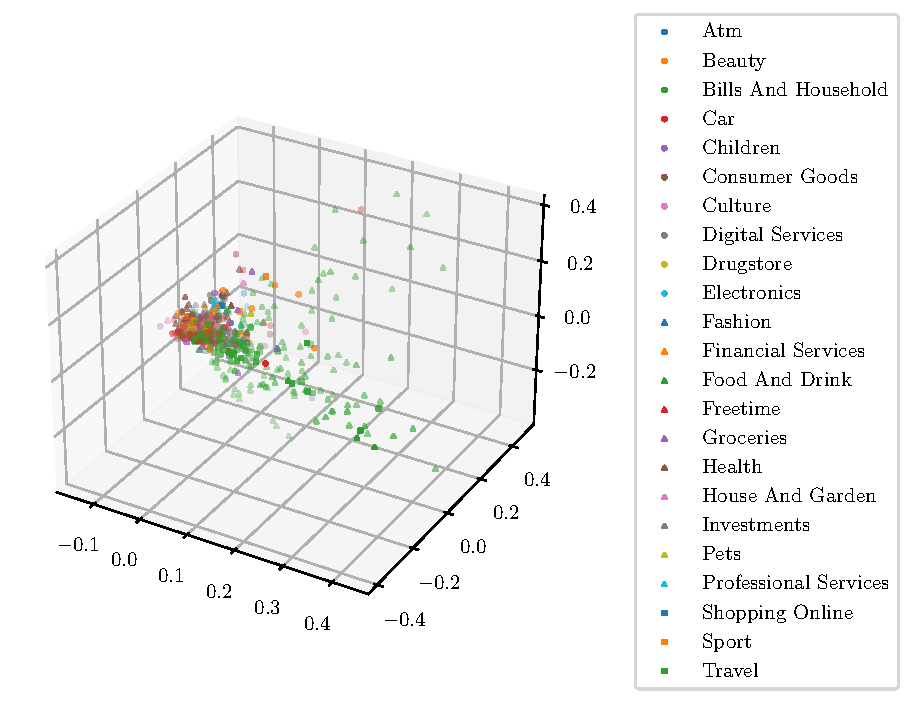
\includegraphics[width=\textwidth]{../img/plot_text_data_all_pca_analysis.pdf}
\caption{Dimensionality reduction with PCA using all data.}
\label{fig:3d_pca}
\end{figure}

\openright
\end{document}
